% Laboratory practice
% 2019-08-08 v. 0.1.0
% Juan Camilo Henao Londono
% Universität Duisburg-Essen
% \documentclass[12pt,a4paper,oneside]{article}
% % Default format
% \documentclass[12pt,twoside]{article}
% % Book format
% \documentclass[12pt, a4paper, twoside]{book}
\documentclass[12pt, a4paper, oneside]{book}
% include files that load packages and define macros
%%%%%%%%%%%%%%%%%%%%%%%%%%%%%%%%%%%%%%%%%
% University Assignment Title Page 
% LaTeX Template
% Version 1.0 (27/12/12)
%
% This template has been downloaded from:
% http://www.LaTeXTemplates.com
%
% Original author:
% WikiBooks (http://en.wikibooks.org/wiki/LaTeX/Title_Creation)
%
% License:
% CC BY-NC-SA 3.0 (http://creativecommons.org/licenses/by-nc-sa/3.0/)
% 
% Instructions for using this template:
% This title page is capable of being compiled as is. This is not useful for 
% including it in another document. To do this, you have two options: 
%
% 1) Copy/paste everything between \begin{document} and \end{document} 
% starting at \begin{titlepage} and paste this into another LaTeX file where you 
% want your title page.
% OR
% 2) Remove everything outside the \begin{titlepage} and \end{titlepage} and 
% move this file to the same directory as the LaTeX file you wish to add it to. 
% Then add \input{./title_page_1.tex} to your LaTeX file where you want your
% title page.
%
%----------------------------------------------------------------------------------------
%	PACKAGES AND OTHER DOCUMENT CONFIGURATIONS
%----------------------------------------------------------------------------------------
\usepackage{ifxetex}
\usepackage{textpos}
% \usepackage{cite}
\usepackage[round]{natbib}
\bibpunct[, ]{(}{)}{;}{a}{}{,}% Citation support using natbib.sty
\renewcommand\bibfont{\fontsize{11}{12}\selectfont}% Bibliography support using natbib.sty
% \usepackage{doi}
\usepackage{kpfonts}
\usepackage[a4paper,hmargin=2.8cm,vmargin=2.0cm,includeheadfoot]{geometry}
\usepackage{ifxetex}
\usepackage{stackengine}
\usepackage{tabularx,longtable,multirow,subfigure,caption}%hangcaption
\usepackage{fncylab} %formatting of labels
\usepackage{fancyhdr}
% \usepackage[svgnames,x11names,table]{xcolor}
\usepackage[dvipsnames]{xcolor}
\usepackage[tight,ugly]{units}
\usepackage{url}
\usepackage{float}
\usepackage[english]{babel}
\usepackage{amsmath}
\usepackage{mathtools}

% Alternative activation, when working with laptop,use draft settings !
\usepackage{graphicx}
% \usepackage[draft]{graphicx}
% Nomenclature
% \usepackage{nomencl}
% \makenomenclature
% %% This code creates the groups
% % -----------------------------------------
% \usepackage{etoolbox}
% \renewcommand\nomgroup[1]{%
%   \item[\bfseries
%   \ifstrequal{#1}{G}{Greek Notations}{%
%   \ifstrequal{#1}{L}{Latin Notations}{%
%   \ifstrequal{#1}{A}{Abbreviations}{}}}%
% ]}
% % -----------------------------------------


\usepackage[colorinlistoftodos]{todonotes}
\usepackage{dsfont}
\usepackage{epstopdf} % automatically replace .eps with .pdf in graphics
%\usepackage{backref}
\usepackage{array}
\usepackage{latexsym}
\usepackage{etoolbox}
\usepackage{enumerate} % for numbering with [a)] format 
\usepackage{blindtext} % Dummy text
\usepackage{ngerman}
\usepackage{listings,lstautogobble}
\usepackage{xparse}
\usepackage[utf8]{inputenc}
\DeclareFixedFont{\ttb}{T1}{txtt}{bx}{n}{12} % for bold
\DeclareFixedFont{\ttm}{T1}{txtt}{m}{n}{12}  % for normal
\usepackage{listings}
\usepackage{color} %red, green, blue, yellow, cyan, magenta, black, white
% \usepackage{subcaption}
\definecolor{mygreen}{RGB}{28,172,0} % color values Red, Green, Blue
\definecolor{mylilas}{RGB}{170,55,241}
\definecolor{deepblue}{rgb}{0,0,0.5}
\definecolor{deepred}{rgb}{0.6,0,0}
\definecolor{deepgreen}{rgb}{0,0.5,0}
\definecolor{codegreen}{rgb}{0,0.6,0}
\definecolor{codegray}{rgb}{0.5,0.5,0.5}
\definecolor{codepurple}{rgb}{0.58,0,0.82}
\definecolor{backcolour}{rgb}{0.95,0.95,0.92}
\definecolor{darkred}{rgb}{0.6,0.0,0.0}
\definecolor{darkgreen}{rgb}{0,0.50,0}
\definecolor{lightblue}{rgb}{0.0,0.42,0.91}
\definecolor{orange}{rgb}{0.99,0.48,0.13}
\definecolor{grass}{rgb}{0.18,0.80,0.18}
\definecolor{pink}{rgb}{0.97,0.15,0.45}
\definecolor{firebrick}{rgb}{0.7,0.13,0.13}
%\usepackage[export]{adjustbox}
%\usepackage{wrapfig}
\usepackage{rotating}
% \usepackage{tikz}
% \usepackage[detect-all]{siunitx}
\usepackage{graphicx}
\usepackage{adjustbox}
\usepackage[T1]{fontenc}
\usepackage{tikz-qtree}                
\usepackage{tikz}
  \usetikzlibrary{shapes,arrows,fit,calc,positioning}
  \tikzset{box/.style={draw, diamond, thick, text centered, minimum height=0.5cm, minimum width=1cm}}
  \tikzset{line/.style={draw, thick, -latex'}}
  \tikzset{every picture/.style={line width=0.75pt}} %set default line width to 0.75pt        
\usepackage{pgfplots}
  \pgfplotsset{compat=1.11,}
% \usepackage[linguistics]{forest}
% \usepackage[titles]{tocloft}
% \usepackage{pythonhighlight}
% \usepackage{minted}
% \usepackage{pygmentex}
\usepackage{notoccite}
% \usepackage[onehalfspacing]{setspace}
% \linespread{1.213}
\usepackage{setspace}
\usepackage{booktabs}
\newcommand{\tabitem}{~~\llap{\textbullet}~~}
\numberwithin{equation}{section}
\usepackage[inline]{enumitem}
\usepackage{titlesec}
\setcounter{tocdepth}{4} 
\setcounter{secnumdepth}{4}
\titleformat{\paragraph}
{\normalfont\normalsize\bfseries}{\theparagraph}{1em}{}
\titlespacing*{\paragraph}
{0pt}{3.25ex plus 1ex minus .2ex}{1.5ex plus .2ex}
% \usepackage{footnotebackref}
% Quick macros to type repeated texts
\setlength{\abovecaptionskip}{0pt} 

\newcommand{\scikit}{}
\def\scikit/{{\tt Scikit-Learn}}

\newcommand\bcitet[1]{\textbf{\citet{#1}}}
\newcommand\bcitep[1]{\textbf{\citep{#1}}}





% for code
% \lstset{frameround=fttt,language=SQL,numbers=left,breaklines=true}
\newcommand{\alen}{.7cm}
\newcommand{\blen}{1.5cm}
\newcommand{\clen}{2.4cm}


% \lstset{
%    frameround=fttt,
%    language=SQL,
%    numbers=left,
%    breaklines=true,
%    keywordstyle=\color{blue}\bfseries, 
%    basicstyle=\ttfamily\color{red},
%    numberstyle=\color{black}
%    }
% \lstMakeShortInline[columns=fixed]|

% \lstset{language=Matlab,%
%     basicstyle=\color{red},
%     breaklines=true,%
%     morekeywords={matlab2tikz},
%     keywordstyle=\color{blue},%
%     morekeywords=[2]{1}, keywordstyle=[2]{\color{black}},
%     identifierstyle=\color{black},%
%     stringstyle=\color{mylilas},
%     commentstyle=\color{mygreen},%
%     showstringspaces=false,%without this there will be a symbol in the places where there is a space
%     numbers=left,%
%     numberstyle={\tiny \color{black}},% size of the numbers
%     numbersep=9pt, % this defines how far the numbers are from the text
%     emph=[1]{for,end,break},emphstyle=[1]\color{red}, %some words to emphasise
%     emph=[2]{word1,word2}, emphstyle=[2]{style},    
% }

% Python style for highlighting
\newcommand\pythonstyle{\lstset{
language=Python,
% morekeywords={self},              % Add keywords here
morekeywords=[1]{,as,assert,nonlocal,with,yield,self,True,False,None,} % Python builtin
morekeywords=[2]{,__init__,__add__,__mul__,__div__,__sub__,__call__,__getitem__,__setitem__,__eq__,__ne__,__nonzero__,__rmul__,__radd__,__repr__,__str__,__get__,__truediv__,__pow__,__name__,__future__,__all__,}, % magic methods
morekeywords=[3]{,object,type,isinstance,copy,deepcopy,zip,enumerate,reversed,list,set,len,dict,tuple,range,xrange,append,execfile,real,imag,reduce,str,repr,}, % common functions
morekeywords=[4]{,Exception,NameError,IndexError,SyntaxError,TypeError,ValueError,OverflowError,ZeroDivisionError,}, % errors
morekeywords=[5]{,ode,fsolve,sqrt,exp,sin,cos,arctan,arctan2,arccos,pi, array,norm,solve,dot,arange,isscalar,max,sum,flatten,shape,reshape,find,any,all,abs,plot,linspace,legend,quad,polyval,polyfit,hstack,concatenate,vstack,column_stack,empty,zeros,ones,rand,vander,grid,pcolor,eig,eigs,eigvals,svd,qr,tan,det,logspace,roll,min,mean,cumsum,cumprod,diff,vectorize,lstsq,cla,eye,xlabel,ylabel,squeeze,}, % numpy / math
keywordstyle=[1]\color{blue},
keywordstyle=[2]\color{blue},
keywordstyle=[3]\color{grass},
keywordstyle=[4]\color{red},
keywordstyle=[5]\color{orange},
% keywordstyle=\color{blue},
emph={MyClass,__init__},          
emphstyle=\color{deepred},                            
backgroundcolor=\color{backcolour},   
commentstyle=\color{codegreen},
numberstyle=\tiny\color{codegray},
stringstyle=\color{codepurple},
basicstyle=\ttfamily\scriptsize,
breakatwhitespace=false,         
breaklines=true,                 
captionpos=b,                    
keepspaces=true,                 
numbers=left,                    
numbersep=5pt,                  
showspaces=false,                
showstringspaces=false,
showtabs=false,                  
tabsize=2,
autogobble = true
}}

% Python environment
\lstnewenvironment{python}[1][]
{
\pythonstyle
\lstset{#1}
}
{}

% Python for external files
\newcommand\pythonexternal[2][]{{
\pythonstyle
\lstinputlisting[#1]{#2}}}

% Python for inline
\newcommand\pythoninline[1]{{\pythonstyle\lstinline!#1!}}

% \lstdefinestyle{mystyle}{
%     backgroundcolor=\color{backcolour},   
%     commentstyle=\color{codegreen},
%     keywordstyle=\color{magenta},
%     numberstyle=\tiny\color{codegray},
%     stringstyle=\color{codepurple},
%     basicstyle=\ttfamily\scriptsize,
%     breakatwhitespace=false,         
%     breaklines=true,                 
%     captionpos=b,                    
%     keepspaces=true,                 
%     numbers=left,                    
%     numbersep=5pt,                  
%     showspaces=false,                
%     showstringspaces=false,
%     showtabs=false,                  
%     tabsize=2,
%     autogobble = true
% }

% Define Pylance color scheme
\definecolor{pylance-purple}{RGB}{136, 0, 137}
\definecolor{pylance-green}{RGB}{49, 133, 80}
\definecolor{pylance-blue}{RGB}{41, 60, 85}
\definecolor{pylance-gray}{RGB}{75, 85, 98}

\lstset{
    language=Python,        % Choose the language
    basicstyle=\ttfamily\scriptsize\color{pylance-blue},  % Font style for code
    keywordstyle=\color{pylance-purple},   % Style for keywords
    commentstyle=\color{pylance-green},     % Style for comments
    stringstyle=\color{pylance-gray},    % Style for strings
    numbers=left,           % Line numbers on the left
    numberstyle=\tiny\color{pylance-gray},  % Style for line numbers
    stepnumber=1,           % Line numbers increment by 1
    numbersep=5pt,          % Distance between line numbers and code
    % basicstyle=\ttfamily\scriptsize,
    backgroundcolor=\color{white}, % Background color for code
    showspaces=false,       % Don't show spaces in code
    showstringspaces=false, % Don't show spaces in strings
    showtabs=false,         % Don't show tabs in code
    % frame=single,           % Frame around code
    rulecolor=\color{pylance-gray},
    tabsize=4,              % Tab size
    captionpos=b,           % Position of captions
    breaklines=true,        % Automatically break lines
    breakatwhitespace=true, % Break lines at white space
    escapeinside={\%*}{*)}, % Define characters for escaping within code
    morekeywords={True, False, None}, % Additional keywords
    autogobble = true
}



\ifxetex
\usepackage{fontspec}
\setmainfont[Scale=.8]{OpenDyslexic-Regular}
\else
% \usepackage[pdftex,pagebackref,hypertexnames=false,colorlinks]{hyperref} % provide links in pdf
\usepackage[pdftex,hypertexnames=false,colorlinks]{hyperref} % provide links in pdf
\usepackage[nameinlink,noabbrev]{cleveref}
\usepackage{doi}
\usepackage{footnotebackref}
\usepackage{tablefootnote} % for table footnotes
\hypersetup{pdftitle={},
  pdfsubject={}, 
  pdfauthor={Hibatul Wafi},
  pdfkeywords={}, 
  pdfstartview=FitH,
  pdfpagemode={UseOutlines},% None, FullScreen, UseOutlines
  bookmarksnumbered=true, bookmarksopen=true, colorlinks,
    % citecolor=NavyBlue,%
    citecolor=black,%
    filecolor=NavyBlue,%
    linkcolor=black,%
    urlcolor=NavyBlue}
  % citecolor=black,%
    % filecolor=black,%
    % linkcolor=black,%
    % urlcolor=black}
\usepackage[all]{hypcap}
\fi

\usepackage{tcolorbox}

% various theorems
\usepackage{ntheorem}
\theoremstyle{break}
\newtheorem{lemma}{Lemma}
\newtheorem{theorem}{Theorem}
\newtheorem{remark}{Remark}
\newtheorem{definition}{Definition}
\newtheorem{proof}{Proof}

% example-environment
\newenvironment{example}[1][]
{ 
\vspace{4mm}
\noindent\makebox[\linewidth]{\rule{\hsize}{1.5pt}}
\textbf{Example #1}\\
}
{ 
\noindent\newline\makebox[\linewidth]{\rule{\hsize}{1.0pt}}
}



%\renewcommand{\rmdefault}{pplx} % Palatino
% \renewcommand{\rmdefault}{put} % Utopia

\ifxetex
\else
\renewcommand*{\rmdefault}{bch} % Charter
\renewcommand*{\ttdefault}{cmtt} % Computer Modern Typewriter
%\renewcommand*{\rmdefault}{phv} % Helvetica
%\renewcommand*{\rmdefault}{iwona} % Avant Garde
\fi

\setlength{\parindent}{0em}  % indentation of paragraph

\setlength{\headheight}{14.5pt}
\pagestyle{fancy}
\newcommand{\changefont}{%
    \fontsize{9}{11}\selectfont
}
\fancyhead[LE,RO]{\changefont \slshape \rightmark} %section
\fancyhead[RE,LO]{\changefont \slshape \leftmark} %chapter
\fancyfoot[C]{\thepage} %footer
% \fancyfoot[EC,OC]{\thepage}
% \fancyfoot[OC,EC]{\sffamily }
% \fancyfoot[ER,OL]{\thepage}
% \fancyfoot[OC,EC]{\sffamily }
%Page no. in the left on
%odd pages and on right on even pages
\renewcommand{\headrulewidth}{0.1pt}
\renewcommand{\footrulewidth}{0.1pt}
\captionsetup{margin=10pt,font=small,labelfont=bf}

% Set pagestyle for front matter
\fancypagestyle{frontmatter}{
  \renewcommand{\headrulewidth}{0pt} % No header line
  \fancyhf{} % Clear header and footer
  \cfoot{\thepage} % Centered page number
}

%--- chapter heading

\def\@makechapterhead#1{%
  \vspace*{10\p@}%
  {\parindent \z@ \raggedright %\sffamily
        %{\Large \MakeUppercase{\@chapapp} \space \thechapter}
        %\\
        %\hrulefill
        %\par\nobreak
        %\vskip 10\p@
    \interlinepenalty\@M
    \Huge \bfseries 
    \thechapter \space\space #1\par\nobreak
    \vskip 30\p@
  }}

%---chapter heading for \chapter*  
\def\@makeschapterhead#1{%
  \vspace*{10\p@}%
  {\parindent \z@ \raggedright
    \sffamily
    \interlinepenalty\@M
    \Huge \bfseries  
    #1\par\nobreak
    \vskip 30\p@
  }}
  

% %%%%%%%%%%%%% boxit
\def\Beginboxit
   {\par
    \vbox\bgroup
	   \hrule
	   \hbox\bgroup
		  \vrule \kern1.2pt %
		  \vbox\bgroup\kern1.2pt
   }

\def\Endboxit{%
			      \kern1.2pt
		       \egroup
		  \kern1.2pt\vrule
		\egroup
	   \hrule
	 \egroup
   }	

\newenvironment{boxit}{\Beginboxit}{\Endboxit}
\newenvironment{boxit*}{\Beginboxit\hbox to\hsize{}}{\Endboxit}



\allowdisplaybreaks

\makeatletter
\newcounter{elimination@steps}
\newcolumntype{R}[1]{>{\raggedleft\arraybackslash$}p{#1}<{$}}
\def\elimination@num@rights{}
\def\elimination@num@variables{}
\def\elimination@col@width{}
\newenvironment{elimination}[4][0]
{
    \setcounter{elimination@steps}{0}
    \def\elimination@num@rights{#1}
    \def\elimination@num@variables{#2}
    \def\elimination@col@width{#3}
    \renewcommand{\arraystretch}{#4}
    \start@align\@ne\st@rredtrue\m@ne
}
{
    \endalign
    \ignorespacesafterend
}
\newcommand{\eliminationstep}[2]
{
    \ifnum\value{elimination@steps}>0\leadsto\quad\fi
    \left[
        \ifnum\elimination@num@rights>0
            \begin{array}
            {@{}*{\elimination@num@variables}{R{\elimination@col@width}}
            |@{}*{\elimination@num@rights}{R{\elimination@col@width}}}
        \else
            \begin{array}
            {@{}*{\elimination@num@variables}{R{\elimination@col@width}}}
        \fi
            #1
        \end{array}
    \right]
    & 
    \begin{array}{l}
        #2
    \end{array}
    &%                                    moved second & here
    \addtocounter{elimination@steps}{1}
}
\makeatother

%% Fast macro for column vectors
\makeatletter  
\def\colvec#1{\expandafter\colvec@i#1,,,,,,,,,\@nil}
\def\colvec@i#1,#2,#3,#4,#5,#6,#7,#8,#9\@nil{% 
  \ifx$#2$ \begin{bmatrix}#1\end{bmatrix} \else
    \ifx$#3$ \begin{bmatrix}#1\\#2\end{bmatrix} \else
      \ifx$#4$ \begin{bmatrix}#1\\#2\\#3\end{bmatrix}\else
        \ifx$#5$ \begin{bmatrix}#1\\#2\\#3\\#4\end{bmatrix}\else
          \ifx$#6$ \begin{bmatrix}#1\\#2\\#3\\#4\\#5\end{bmatrix}\else
            \ifx$#7$ \begin{bmatrix}#1\\#2\\#3\\#4\\#5\\#6\end{bmatrix}\else
              \ifx$#8$ \begin{bmatrix}#1\\#2\\#3\\#4\\#5\\#6\\#7\end{bmatrix}\else
                 \PackageError{Column Vector}{The vector you tried to write is too big, use bmatrix instead}{Try using the bmatrix environment}
              \fi
            \fi
          \fi
        \fi
      \fi
    \fi
  \fi 
}  
\makeatother

\robustify{\colvec}

%%% Local Variables: 
%%% mode: latex
%%% TeX-master: "notes"
%%% End: 
 % various packages needed for maths etc.


\input{00_setup/notation.tex} % short-hand notation and macros

\begin{document}
% \thispagestyle{empty}

% \newcommand{\HRule}{\rule{\linewidth}{0.5mm}} % Defines a new command for the horizontal lines, change thickness here

% % Logo
% \includegraphics[width=\columnwidth]{02_figures/logo_en.jpg}
% \vspace{1cm}

% \begin{center} % Center remainder of the page

% % Heading section
% \textsc{\LARGE University of Duisburg-Essen}\\[1cm] 
% \textsc{\Large Chair of Transport Systems and Logistics}\\[1cm]
% %\textsc{\large Advanced Laboratory}\\[1cm]

% % Title
% \HRule \\[0.4cm]
% {\Huge \bfseries Modelling and optimization of ship’s fuel consumption using Random Forest Regression (RFR) }\\[0.5cm] % Title of your document
% {\Large Modellierung und Optimierung des Treibstoffverbrauchs von Schiffen mittels Random Forest Regression (RFR)}
% \HRule \\[2cm]

% % Author

% \begin{minipage}{0.4\textwidth}
% \begin{flushleft} \large
% 	\emph{Author:}\\
% 	Hibatul Wafi\\
%     3021919\\
% %    \textbf{Group \#}
% 	\end{flushleft}
% 	\end{minipage}
% ~
% \begin{minipage}{0.4\textwidth}
% \begin{flushright} \large
% 	\emph{Supervisor:} \\
% 	M. T. Muhammad Fakhruriza Pradana
% \end{flushright}
% \end{minipage}\\
% \vspace{1cm}
% \makeatletter
% \vspace{1cm}
% {\large Summer semester 2023} \\
% {\large \@date}
% \end{center}

\def\whatIsIt{Master Thesis}
\def\title{Modelling and optimization of ship's fuel consumption using Random Forest Regression (RFR)}
\def\fakultaet{Faculty of Engineering}

\def\author{Hibatul Wafi}
% \def\addrLineEins{Muster Straße 1}
% \def\addrLineZwei{PLZ, Ort}
\def\matrikelNr{3021919}

\def\location{Duisburg}
\def\date{04.05.2023}

\def\betreuer{M. T. Muhammad Fakhruriza Pradana}
\def\ersterGutachter{Prof. Dr.-Ing. B. Noche}
\def\zweiterGutachter{Dr.-Ing. Alexander Goudz}
\def\fach{ISE General Mechanical Engineering}
\def\semester{Summer semester 2023}

\begin{titlepage}
	\vspace*{-6em}
	\hspace{-3.5em}
	\includegraphics[scale=0.2]{02_figures/ude.jpg}
	\vspace*{\fill}
			
	\begin{center}
		{\Large\bfseries \whatIsIt}\\
		\vspace*{\fill}
		on the topic of\\
		\vspace*{\fill}
		{\huge\bfseries \title} \\
		\vspace*{\fill}
		Submitted to the \fakultaet\\
		of University Duisburg Essen\\
		\vspace*{\fill}
		by\\
		\vspace*{\fill}
		{\large\bfseries\author} \\
		% \addrLineEins\\
		% \addrLineZwei\\
		{\large\bfseries\matrikelNr} \\
	\end{center}
	
	\vspace*{\fill}
	
	\begin{tabular}{ll}
		Betreuer: & \betreuer\\
		1. Gutachter: & \ersterGutachter\\
		2. Gutachter: & \zweiterGutachter\\
		Studiengang: & \fach \\
		Studiensemester: & \semester \\
		Datum: & \date
	\end{tabular}
	
\end{titlepage}
\pagebreak
\frontmatter
\pagestyle{plain}
\cleardoublepage
\phantomsection
\chapter*{Abstract}
\addcontentsline{toc}{chapter}{Abstract}

% There has been various efforts to model energy efficient operation of shipping operations which is necessitated by the volatility of bunker fuel price and stringent environmental regulations within the maritime industry. It is widely regarded that ship speed is one of the most influential factors impacting bunker fuel consumption. Machine learning models have demonstrated promising capabilities in predicting fuel consumption (FOC). However, the more powerful machine learning model is comparatively complex and lacking in interpretability, making it challenging to comprehend the rationale behind their decisions. Additionally, in some cases, these models could potentially generate predictions that are not aligned with established knowledge of ship operations. The success of these models is also heavily reliant on the quality and quantity of the data available.\\

% Therefore, an intuitive, data-driven modelling approach that considers varying ship states and environmental conditions to predict fuel consumption is proposed in this study. To ensure the abundance of data during modelling, this thesis combines Automatic Identification System data and weather data. Grey Box Modelling approach is implemented for FOC prediction, which divides the prediction of ship speed and FOC into two stages. The prediction of speed over ground utilises Random Forest Regressor, a tree-based machine learning approach that offers a certain degree of intuitiveness. Consequently, the FOC prediction based on predicted speed employs empirical formula by Holtrop-Mennen, ensuring adherence to established physical knowledge of a vessel.\\

% In the case study presented in this thesis, the optimal SOG prediction yields a mean absolute percentage error of $3.94\%$ knots with $R^2$ score of $93.41\%$. Then the consequent FOC prediction using the predicted achieved $R^2$ score of $86.57\%$ and mean absolute percentage error stands at $12.06\%$. Improvements in predictive capabilities could potentially be attained by using Extra Tree Regressor. Nonetheless, these results indicated the viability of the proposed methodology for forecasting energy-efficient ship operations.\\

Efforts to model energy-efficient operation of shipping operations using machine-learning methods have emerged due to volatile bunker fuel prices and stringent environmental regulations. It is widely regarded that ship speed is one of the most influential factors impacting ships' fuel oil consumption and as such, accurate modelling of ship speed is paramount to ensure the accuracy of subsequent FOC prediction.\\

This study proposes an intuitive data-driven modelling approach, integrating Automatic Identification System and weather data for modelling of ship states and environmental conditions' impact on FOC. Grey Box Modelling approach divides the speed and FOC prediction into stages, the first stage involves the prediction of speed over ground using Random Forest Regressor. Consequently, the FOC prediction based on predicted speed employs the empirical formula by Holtrop-Mennen, maintaining adherence with established vessel knowledge.\\
  
In the presented case study, optimised SOG prediction achieves $3.94\%$ mean absolute percentage error (MAPE) and $93.41\%$ $R^2$ score. Subsequent FOC prediction from estimated speed yields $86.57\%$ $R^2$ and $12.06\%$ MAPE. The results affirm the proposed approach's viability in predicting energy-efficient ship operations.\\


\textbf{\small Keywords: Energy efficient operation, Random Forest Regression, Ship speed prediction, Fuel consumption prediction, Grey Box Model, AIS}.
\newpage
\cleardoublepage
\phantomsection
\chapter*{Acknowledgments}
\addcontentsline{toc}{chapter}{Acknowledgments}

To my family, who makes everything worthwhile

\newpage
\cleardoublepage
\phantomsection
\addcontentsline{toc}{chapter}{Table of Contents}
\tableofcontents
\newpage
\cleardoublepage
\phantomsection
\addcontentsline{toc}{chapter}{List of Tables}
\listoftables
\newpage
\cleardoublepage
\phantomsection
\addcontentsline{toc}{chapter}{List of Figures}
\listoffigures
\newpage
\cleardoublepage
\phantomsection

%====================================================================================
\chapter*{Nomenclature}
\addcontentsline{toc}{chapter}{Nomenclature}

%====================================================================================
\section*{Symbols with Latin letters}
\label{symbols_latin}
\renewcommand{\arraystretch}{1.3}

\begin{longtable}[l]{>{$}l<{$}l>{$}l<{$}}
\textbf{Symbol}&\textbf{Denomination}&\textbf{SI Unit}\\[0.5ex]\hline
\endfirsthead%
\textbf{Symbol}&\textbf{Denomination}&\textbf{SI Unit}\\[0.5ex]\hline
\endhead%
    A_E / A_O   & Propeller expanded area ratio & - \\%
    A_{BT}      & Transverse area of bulbous bow & m^2 \\%
    A_L         & Lateral plane area            & m^2 \\%
    A_T         & Immersed transom area         & m^2 \\%
    A_V         & Area of ship and cargo above waterline & m^2 \\%
    A_W         & Waterline area                & m^2 \\%
    B           & Breadth                       & m \\%
    C_B         & Block coefficient             & - \\%
    C_{D_{TH}}  & Drag coefficient of thruster tunnel & - \\%
    C_F         & Frictional Coefficient        & - \\%
    C_M         & Midship coefficient           & - \\%
    C_P         & Prismatic coefficient         & - \\%
    C_{WP}      & Waterplane area coefficient   & - \\%
    CD_l        & Drag coefficient for beam wind & - \\%
    CD_t        & Drag coefficient for headwind & - \\%
    D           & Propeller diameter            & m \\%
    d_{TH}      & Diameter of bow thruster tunnel & m \\%
    Fr          & Froude Number                 & - \\%
    g           & Gravity constant              & kg/ms^2 \\%
    \overline{H}& Mean wave height              & m \\%
    H_{1/3}     & Significant wave height       & m \\%
    H_{10}      & Highest ten percent of wave   & m \\%
    H_{max}     & Maximum wave height           & m \\%
    H_{swell}   & Swell wave height             & m \\%
    H_{windwave}& Wind wave height              & m \\% 
    h_B         & Height of centre $A_{BT}$ above basis & m \\%
    i_E         & Half angle of waterline entrance & \text{°} \\%    
    J           & Cost function                 & - \\%
    k           & Form factor                   & - \\%
    k_{2_i}     & Appendage form factor         & - \\%    
    \text{k}_n  & Feature $n$ of ML model       & - \\%
    \ell_{CB}   & Longitudinal Centre of buoyancy & - \\%
    L_{BWL}     & Length of bow in the waterline & m \\%
    L_{WL}      & Waterline length              & m \\%
    L_{PP}       & Length between perpendicular  & m \\%
    L_R         & Length of run                 & m \\%
    n           & Data point(s)                    & - \\%
    P_b         & Brake power                   & kW \\%
    P_e         & Effective power               & kW \\%
    R_A         & Correlation resistance        & kN \\%
    R_{AA}      & Additional resistance due to wind & kN \\% 
    R_{AW}      & Additional resistance due to wave & kN \\%
    R_{APP}     & Appendage Resistance          & kN \\%
    R_B         & Resistance of bulbous bow     & kN \\%    
    R_F         & Frictional Resistance         & kN \\%
    R_{CALM}    & Calm water resistance         & kN \\%
    R_{TOTAL}   & Total Resistance              &\text{$kN$} \\%
    R_{TR}      & Transom Resistance            & kN \\%
    R_W         & Wave resistance               & kN \\%
    R^2         & Coefficient of Determination  & - \\%
    Re          & Reynolds number               & - \\%
    \text{S}_i  & Partition space $i$           & - \\%
    S           & Wetted surface of bare hull   & m^2 \\%
    S_{App}     & Wetted surface of appendages  & m^2 \\%
    t           & Thrust deduction fraction     & - \\%
    \text{t}_k  & Tree threshold $k$            &- \\%
    T           & Draught                       & m \\%
    T_A         & Moulded draught at aft perpendicular & m \\%
    T_F         & Moulded draught at forward perpendicular & m \\%
    \text{T}_p  & Spectral peak period          & s \\%    
    \text{T}_f  & Spectral peak period of fully developed sea & s \\%
    u           & Apparent wind velocity        & m/s \\%
    u_{TW}      & True wind velocity w.r.t to bow & m/s \\%
    u_{W}       & Wind velocity                 & m/s \\%
    V           & Displacement volume           & m^3 \\%
    v           & Speed                         & m/s  \\%
    v_C         & Current Speed                 & m/s \\%
    v_G         & Speed Over Ground             & m/s \\%
    v_S         & Speed Through Water           & m/s \\%
    w           & Wake fraction                 & - \\%
    y           & Response variable             &- \\%
    \hat{y}     & Mean of response variable     & - \\%

\end{longtable}
\vspace{5ex}

%====================================================================================
\section*{Symbols with Greek letter}

\begin{longtable}[l]{>{$}l<{$}l>{$}l<{$}}
\textbf{Symbol}&\textbf{Denomination}&\textbf{SI Unit}\\[0.5ex]\hline%
\endfirsthead%
\textbf{Symbol}&\textbf{Denomination}&\textbf{SI Unit}\\[0.5ex]\hline%
\endhead%
\renewcommand{\arraystretch}{1.3}
 \label{symbols_greek}
     \alpha &   Heading angle                &  \text{°} \\%
     \beta  &   True wind angle              &  \text{°}  \\%
     \gamma &   True north current direction &  \text{°}   \\%
     \delta &   Cross force parameter        & - \\%
     \varepsilon & Apparent wind angle       & \text{°} \\%
     \eta_s &   Shaft efficiency             & - \\%
     \eta_h &   Hull efficiency              & - \\%
     \eta_r &   Rotative efficiency          & - \\%
     \eta_o &   Open water efficiency        & - \\%
     \eta_{TOTAL} & Total efficiency         & - \\%
     \nu    &   Kinematic viscosity          & m^2/s \\%
     \rho   &   Density                      & kg/m^3 \\%   
     \tau   &   Time                         & ss/hh/dd \\%
     \varphi & True north wind direction     & \text{°} \\%
     



\end{longtable}

%====================================================================================
\section*{Abbreviations}

\begin{longtable}[l]{>{}l<{}l}
  \textbf{Abbreviation} & \textbf{Denomination} \\[0.5ex] \hline%
  \endfirsthead%
  \textbf{Abbreviation} & \textbf{Denomination} \\[0.5ex] \hline%
  \endhead%
\renewcommand{\arraystretch}{1.4}\label{abbreviations}
&\\%
AB          & AdaBoost\\%
ADLM        & Automatic Data Logging System\\% 
(T/S)-AIS   & (Terrestrial/Sattelite)-Automatic Identification System\\%
ANN         & Artificial Neural Network\\%
BBM         & Black Box Model\\%
CART        & Classification and Regression Tree\\%
CMEMS       & Copernicus Marine Environment Monitoring Service \\%  
COG         & Course Over Ground \\% 
DMA         & Danish Maritime Authority \\%
DS          & Data set \\%
DT(R)       & Decision Tree (Regressor)\\%
ECMWF       & European Centre for Medium-Range Weather Forecast\\%
EEOI        & Energy Efficient Operational Indicator\\%
ET(R)       & Extra Tree (Regressor)\\%
EV          & Explained Variance \\%
FOC         & Fuel Oil Consumption\\%
GB          & Gradient Boosting\\%
GBM         & Grey Box Model \\%
GHG         & Green House Gas \\%
GPS         & Global Positioning System\\% 
GT          & Gross Tonnage\\%
IMO         & International Maritime Organization\\%
ITTC        & International Towing Tank Conference \\%
IQR         & Interquartile Range \\%
KNN         & K-Nearest Neighbour\\%
LASSO       & Least Absolute Shrinkage and Selection Operator\\%
LB          & Light Gradient Boosting Machine\\%
(M)LR       & (Multiple) Linear Regression\\%
MAD         & Median Absolute Deviation \\%
MAE         & Mean Absolute Error \\%
MAPE        & Mean Absolute Percentage Error \\%
ML          & Machine Learning\\%
MLP         & Multi Level Perceptron\\%
MMSI        & Maritime Mobile Service Identity \\%
MSE         & Mean Square Error\\%
OPEX        & Operational Expenses\\%
RF(R)       & Random Forest (Regressor)\\%
RMSE        & Root Mean Square Error\\%
RPM         & Revolution per Minute\\%
SEEMP       & Ship Energy Efficiency Management Plan\\%
SFOC        & Specific Fuel Oil Consumption \\%
SOG         & Speed Over Ground \\%
SOLAS       & International Convention for Safety of Lives at Sea\\%
STW         & Speed Through Water \\%
SVR         & Support Vector (Regressor)\\%
TWA         & True Wind Angle\\%
VHF         & Very High Frequency\\%
WBM         & White Box Model\\%
XG          & eXtreme Gradient Boosting\\%

\end{longtable}

\setlength{\extrarowheight}{0pt}

% \newpage
% \newcommand{\listequationsname}{List of Equations}
\newlistof{myequations}{equ}{\listequationsname}
\newcommand{\myequations}[1]{% 
\addcontentsline{equ}{myequations}{\protect\numberline{\theequation}#1}\par}
% \addcontentsline{equ}{myequations}{\protect\numberline{\theequation}#1}\par}

\listofmyequations
% {\setstretch{1}
\mainmatter
\pagestyle{fancy}
\newpage
\chapter{Introduction} \label{chp:introduction}

Marine industry stakeholders are actively pursuing research on efficient ship operation. This research direction is motivated by the increasing price of fuel oil and stricter environmental regulations. The fuel aboard a ship is referred to as ``bunkers'' and accounts for a substantial portion of the vessel's operational expenses (OPEX). It is known that bunker fuel takes up more than 50\% of voyage costs and constitutes up to 75\% of the ship's total operating cost. It can be inferred that energy-efficient ship operations that could reduce fuel consumption translate to an increase in profitability \bcitep{Stopford.2009,Ronen.2011,Bialystocki.2016}. Furthermore, efficient operation also means the reduction of Greenhouse Gas Emissions (GHG). The most recent report by International Maritime Organisation indicated that GHG emissions from shipping make up 2.51\% of global emissions \bcitep{IMO.2020}. This mutual motivation aligns economic benefits with environmental compliance.\\

With that, maritime industry stakeholder actively searches for methods to ensure energy-efficient operation. Two approaches are considered, namely technical solutions and operational solutions. Technical solutions involve modification to the vessel's structure and power system. But these solutions are expensive, and it requires engineering innovations \bcitep{Yan.2021,Li.2022}. Because of this, stakeholders look for cheaper solutions to achieve energy-efficient operations. The answer for an inexpensive approach lies in the optimisation of operational measures, it carries less cost, and it does not require initial investments. Several recommended solutions for energy-efficient operation can be found in Ship Energy Efficiency Management Plan (SEEMP).\\ 

Significant emphasis is given in this study on the optimisation of ship speed as it is widely considered that ship speed has a substantial impact on fuel consumption. Different studies indicated that fuel consumption is correlated through a third-order, non-linear function of the ship speed \bcitep{Wang.2012,Ronen.2011,Psaraftis.2013,Du.2019}. The significant impact of ship speed on fuel consumption is further supplemented by reports and studies stating that reducing ship speed by about $2-3$ knots could halve the operating cost of shipping companies \bcitep{Stopford.2009,Wijnolst.2009}. Hence, energy-efficient operation is commonly achieved through the practice of slow steaming by shipping industry operators. \\

While inexpensive, optimising operational measures is not an easy and trivial task. Several factors ranging from vessel operational performance to varying weather conditions make it challenging to model the ship speed. Some fuel consumption models, which are based on historical data and ship parameters, lack generalisation capabilities, and it is sensitive towards noisy data. To address this problem, recent research turns towards data-driven approach i.e. machine learning (ML) approach to predict ship speed and fuel consumption. These studies reported success in their modelling, citing good generalisation capability and low prediction errors. Despite these successes, maritime experts find it difficult to accept models based on data-driven approach, as some data-driven models are complex as well as unintuitive and in some cases can violate basic physical knowledge of the vessel. The performance of the data-driven model is also greatly dependent on both data quantity and quality \bcitep{Yan.2021,Gkerekos.2019}.\\      

As such, prompted by volatility and ever-increasing bunker fuel price, developing a model that could accurately predict Fuel Oil consumption (FOC) could prove to be useful to maritime industry stakeholders. As stakeholders could make critical economical decisions at the most opportune moment without violating the stringent environmental regulations. \\

\section{Thesis objectives}\label{sec:objectives}

This thesis proposes an intuitive, data-driven modelling approach that considers varying ship states and environmental conditions to predict the fuel consumption of a vessel. To ensure the abundance of data during modelling, this thesis utilise data fused between Automatic Identification System (AIS) and weather data.\\

To achieve this, Grey Box Model (GBM) approach is selected. ML approach using tree-based regressor is considered to provide a certain degree of intuitiveness to predict speed over ground (SOG) over different journey periods using fused AIS and weather data. Predicted SOG is then converted to actual ship speed i.e. Speed Through Water (STW). STW will be used as the input for the modelling of Fuel Oil Consumption (FOC), which is carried out through Holtrop-Mennen estimation method \bcitep{Holtrop.1978,Holtrop.1982,Holtrop.1984}, a power estimation method based on hydrodynamic laws which consider resistance forces exerted by environmental conditions.\\

\pagebreak

The following Research Questions (RQs) could be raised during the development of the model :

\begin{itemize}
    \item \textbf{RQ1}: What are the steps that should be taken to optimise the predictive performance of the model?
    \item \textbf{RQ2}: Is it feasible to fuse AIS data and meteorological data to accurately predict the ship's SOG and subsequently FOC of the ship?
    \item \textbf{RQ3}: Which approximations and empirical equations are suitable to estimate the resistance forces required to estimate the power required by the ship? 
\end{itemize} 

\section{Thesis Boundaries}\label{sec:boundaries}

The following research boundaries are set throughout this thesis:

\begin{itemize}
    \item The weather information and AIS data are assumed to be true. Any uncertainties from AIS data and weather data are neglected. 
    \item The focus of this work is a detailed study of the performance and possible optimisation configuration of different tree-based predictors for SOG. As such, an exhaustive comparison study between different types of machine learning models will not be performed.
    \item In the case study, the approximation for incomplete ship parameters and dimensions is based on a similar type of ship with nearly identical dimensions. 
\end{itemize}

\section{Thesis Contributions}\label{sec:contributions}

The GBM approach using the fusion of AIS data and weather data provides the following contributions : 

\begin{itemize}
    \item Economical and independent data source.
    \item Robust modelling approach that requires minimal data pre-processing and minimal model configuration.
    \item Comprehensible model that adheres to physical principles and hydrodynamic laws of the vessel.  
\end{itemize} 

\pagebreak

\section{Thesis Structure}\label{sec:structure_thesis}

The thesis is organised with the following structure:\\

\textbf{\Cref{chp:introduction}} introduces the problem statement and described the objective and boundaries of the thesis. The novelty of this thesis is declared in this chapter.\\

\textbf{\Cref{chp:theory}} explains the fundamental aspects of the methodologies used to develop the Black Box Model (BBM) and the White Box Model (WBM). \Cref{sec:litreview} includes literature review of relevant past and present research. The fundamentals of the tree-based model will be discussed in \Cref{sec:tree_intro}, basic explanation of the parameters used in AIS and weather data will be given in \Cref{sec:ais_theo} and \Cref{sec:weather_theo}. \Cref{sec:holtrop_mennen_calc} presents the empirical formulas and parameters used to estimate fuel consumption used by the ship based on various literature studies.\\ 

\textbf{\Cref{chp:method}} discusses the methodology used to develop tree-based model used for SOG prediction. The discussion comprises analysis of training data, feature selection and reduction and selection of tuning parameters of the model. The methodology to estimate resistance for ship power estimation will be discussed in this chapter as well.\\ 

\textbf{\Cref{chp:result_and_discussion}}, the GBM model will be evaluated using appropriate performance metrics and their effectiveness will be discussed. The review of the strength and limitations concerning the GBM method will be discussed here.\\

\textbf{\Cref{chp:outlook}} The summary of this study and reflections on the research process will be presented here. 




 





%\begin{figure}[h]
%    \centering
%    \includegraphics[width=0.50\textwidth]{02_figures/logo_en.jpg}
%    \caption{A nice plot}
%    \label{fig:mesh1}
%\end{figure}


\newpage
\section{Theoretical Background} \label{theory}

The literature review in \Cref{litreview} presents past and present research on utilisation of machine learning method to achieve energy efficient operation. The concept of modelling ship operation using machine learning model is explained in \Cref{ship_modelling}. Performance of random forest as predictor in previous research are discussed in \Cref{rf_performance}. Brief conclusion of the literature review is presented in \Cref{lit_review_conclusion}.\\

\subsection{Literature Review}\label{litreview}

\subsubsection{Modelling Approach for Ship Operation}\label{ship_modelling}

The work by Yan et al. \cite{Yan.2021} provides a thorough review of the different attempts that have been made by different authors to predict different parameters of ship's operation, this includes ship's fuel consumption. Per definition by Haranen et al. \cite{MichaelHaranen.2016}, the modelling of ship operation is categorised into White Box Model (WBM), Black Box Model (BBM) and Grey Box Model (GBM). Machine learning approach is categorised as BBM, BBM approach is defined as purely data driven approach requiring no prior knowledge about the ship operation. The literature review by Yan et al. \cite{Yan.2021} indicated that about $42\%$ of the research utilised BBM model based on machine learning approach.\\ 

Yan et al. \cite{Yan.2021} elaborated further in their work, that BBMs in general have a good fitting ability for unseen data. BBMs based on machine learning model are able to generalise better compared to BBMs based on statistical modelling. With increasing amount of data, better generalisation performance and handling noisy of data should be expected in a BBM model. However, for this same reason, the quality of BBM model is highly dependent on data quantity and quality. BBM model are also generally complex making it challenging to analyse and explain. Shipping industry experts also are having difficulty accepting models that violate the domain knowledge.\\   

From the work of Yan et al. \cite{Yan.2021}, it can be concluded that model accuracy and appropriateness is a significant factor that should be considered when modelling. The model should obey shipping domain knowledge and an intuitive model will help shipping experts analyse its accuracy. For this reason, tree-based model will be considered as it is known for its intuitiveness and interpretability \cite{Breiman.2017}. Breiman et al.\cite{Breiman.2001} even claimed that random forest is the ``most interpretable'' and ``most accurate''. With that,\Cref{rf_performance} will focus on predictive performance of random forest against different machine learning model on different data types and data source. \\

\subsubsection{Use of AIS Data for Scientific Research}\label{ais_use}

Apart from its intended use as collision avoidance system AIS data have seen potential usage in the field of scientific research. In the third Green House Gas (GHG) study by Smith et al.\cite{T.W.P.Smith.2015}, uses AIS to estimate global shipping emission inventories. Rakke \cite{Rakke2016} proposed a methodology termed ECAIS to calculate ship emissions based on the fuel consumption from AIS data. Through Holtrop-Mennen approximation and literature approximation, the ship's power propulsion can be determined which is subsequently used to predict specific fuel consumption. Wen et al. \cite{Wen.2017} attempted to minimise the Energy Efficiency Operational Indicator (EEOI) using green routing. Recent research by Kim et al. \cite{Kim.2020b} used publicly accessible AIS data, ship static data and environmental data to estimate EEOI  without requiring the actual FOC. The study used big data technology as public data are of large capacity. Generally, the study using AIS data is done to achieve independence from the need to use commercial database. The detail of AIS data will be discussed in \Cref{ais_theo}\\  

\subsubsection{Prediction Performance of Random Forest}\label{rf_performance}

Majority of the BBM approach based on ML is dominated by ANN \cite{Yan.2021}. However, there are literatures that considered decision tree-based modelling approach to predict fuel consumption. Some example of decision tree based modelling include Decision Tree (DT), Random Forest (RF) and Extra Tree (ET). Soner et al. \cite{Soner.2018} implemented tree-based model, which include bagging, random forest (RF), and bootstrap. In their work, they used data captured from onboard sensors of a ferry to predict speed through water and fuel consumption per hour. From the test dataset, the random forest model described root mean square error (RMSE) of $0.34$ Knots during its prediction of Speed Through Water (STW). Yan et al. \cite{Yan.2020} used random forest (RF) model to minimise fuel consumption for a voyage of a dry bulk ship. The model use ship operational data and sea and weather data from noon report and EMCWF. The prediction performance report from this literature reported mean absolute percentage error (MAPE) of $7.91\%$.\\      

The research by Gkerekos et al. \cite{Gkerekos.2019} highlighted the performance of different machine learning models to predict ship's fuel consumption per day using both noon data and automated data logging and monitoring (ADLM) system from a bulk carrier. This research concludes that tree based model displayed good prediction performance on both noon data and sensor based data. Using default parameters, RF model obtained $R^2$ score of $87.55\%$ and $96.26\%$ for noon-data datasets and sensor-based data respectively. It is also noted that it that the data from a 3-month period in ADLM system would be sufficient to create a model with better performance than the model generated by noon data from a collection period of 2.5 year. This literature also concluded that automatic sensor-based data have the potential to increase the model accuracy score, $R^2$, by $5-7\%$ across different machine learning models.\\

Li et al. \cite{Li.2022} performed more extensive research on the effects of data fusions between meteorological data, ship voyage data and AIS data on different machine learning models to predict the ship's FOC. This research highlighted the advantage of fusing meteorological data and ship voyage data. The evaluation on different model performance indicated that RF are among preferable model candidate that could be used in commercial scale due to its good prediction capability and robustness against different datasets. The findings in this research reported that $R^2$ score are above $96\%$ when deployed on the best datasets and achieved $R^2$ score in range between $74\% - 90\%$ over test data. This literature also exhibited the robustness of RF, as it attained the lowest standard deviation at $0.015$ of the $R^2$ score when evaluated against random splits of datasets.\\

Abebe et al. \cite{Abebe.2020} used different approach in their research by predicting the ship's Speed Over Ground (SOG) instead of FOC. In this work, AIS data and noon-report weather data from 14 tracks and 62 ships are used for the SOG prediction. The observation showed that RF model achieved RMSE of $0.25$ knots, while using $489$ seconds for training. Decision tree achieved RMSE of $0.36$ knots, taking up $52$ seconds for training. This shows that RFR outperforms DTR at cost of computational power.\\

\subsubsection{Conclusion of Literature Review}\label{lit_review_conclusion}

This literature review described the capability of Random Forest Regressor to predict fuel consumptions and ship speed, irrespective of data source and type of data used. Promising results from different performance measures across different literatures indicated the capability random forest model as predictor. As such, this thesis aims to find optimisation possibilities to extract maximum prediction performance from random forest. Due to the nonlinear, third order function estimate of fuel consumption \cite{Ronen.1982,Ronen.2011}. Accurate prediction of ship speed is paramount to ensure optimal ship operation resulting in increase of profitability. 

\subsection{Tree-based model}\label{tree_intro}

Random forest belongs to the family of tree-based model and its functional principle stems from decision tree. Decision tree is a non-parametric model that can perform both classification and regression tasks for discrete variable and continuous variable. It is a powerful algorithm, capable of fitting complex datasets. Tree-based model requires very little to no data pre-processing \cite{Geron.2019,Hastie.2009}. To grasp the concept of random forest, The principle working of decision tree will be introduced in depth in \Cref{dt_theo}. It is then followed by \Cref{rf_theo} which presents the principle function behind random forest. Brief explanation for Extra-Trees, method introduced to further improvise random forest, will be presented in \Cref{et_theo}.\\

\subsubsection{Decision Tree}\label{dt_theo}

Decision tree is a white box model\footnote{This is not to be interchanged with the definition described by Haranen et al. \cite{MichaelHaranen.2016} regarding modelling of ship operation.} \cite{Geron.2019}. In machine learning sense, this means that the model is intuitive, and the structure of the model is interpretable. Thus, the structure of the model can be analysed in detail. To train Decision Trees, {\tt Scikit-Learn} \cite{FabianPedregosa.2011} uses the \emph{Classification and Regression Tree} (CART) algorithm \cite{Breiman.2017}. Partition space shown by \Cref{fig:partitionspace} are used to illustrate the decision of CART algorithm. This process can be alternatively represented by the binary tree of \Cref{fig:partitiontree}, observation that satisfies the condition are assigned to the left branch and the opposite is assigned to the right branch. The binary tree representation can be especially helpful when multiple input variables are involved, as the responses can be represented by a single tree \cite{Hastie.2009}.\\

\begin{figure}[h]
\centering
\begin{minipage}[b]{.5\textwidth}
    \centering
    \begin{tikzpicture}[x=0.75pt,y=0.75pt,yscale=-1,xscale=1]
    %uncomment if require: \path (0,433); %set diagram left start at 0, and has height of 433
    
    %Shape: Square [id:dp5731268858272198] 
    \draw   (180,110) -- (370,110) -- (370,300) -- (180,300) -- cycle ;
    %Straight Lines [id:da615072570759449] 
    \draw    (250,110) -- (250,300) ;
    %Straight Lines [id:da8002566967918264] 
    \draw    (300,110) -- (300,300) ;
    %Straight Lines [id:da4409034763483005] 
    \draw    (180,230) -- (250,230) ;
    %Straight Lines [id:da07514682530914596] 
    \draw    (300,170) -- (370,170) ;
    
    % Text Node
    \draw (131,192.4) node [anchor=north west][inner sep=0.75pt]    {$X_{2}$};
    % Text Node
    \draw (261,340.4) node [anchor=north west][inner sep=0.75pt]    {$X_{1}$};
    % Text Node
    \draw (157,222.4) node [anchor=north west][inner sep=0.75pt]    {$t_{2}$};
    % Text Node
    \draw (201,252.4) node [anchor=north west][inner sep=0.75pt]    {$R_{1}$};
    % Text Node
    \draw (201,162.4) node [anchor=north west][inner sep=0.75pt]    {$R_{2}$};
    % Text Node
    \draw (268,192.4) node [anchor=north west][inner sep=0.75pt]    {$R_{3}$};
    % Text Node
    \draw (321,132.4) node [anchor=north west][inner sep=0.75pt]    {$R_{4}$};
    % Text Node
    \draw (321,220.4) node [anchor=north west][inner sep=0.75pt]    {$R_{5}$};
    % Text Node
    \draw (241,310.4) node [anchor=north west][inner sep=0.75pt]    {$t_{1}$};
    % Text Node
    \draw (291,312.4) node [anchor=north west][inner sep=0.75pt]    {$t_{3}$};
    % Text Node
    \draw (381,162.4) node [anchor=north west][inner sep=0.75pt]    {$t_{4}$};
    
    \end{tikzpicture}
    
    \captionof{figure}{Example of partition space \cite{Hastie.2009}} 
    \label{fig:partitionspace}
\end{minipage}%
\begin{minipage}[b]{.5\textwidth}
    \centering
    \begin{tikzpicture}
        \tikzset{level distance=65pt,sibling distance=10pt,edge from parent/.style=
        {draw,edge from parent path={(\tikzparentnode.south)
                                -- +(0,-8pt)
                                -| (\tikzchildnode)}}}
    \Tree [.$X_1\leq t_1$ [.$X_2\leq t_2$ [.$R_1$ ] [.$R_2$ ] ]
        [.$X_1\leq t_3$ [.$R_3$ ]
        [.$X_2\leq t_4$ [.$R_4$ ] [.$R_5$ ] ] ] ]
    \end{tikzpicture}
    \captionof{figure}{Example of partition tree \cite{Hastie.2009}} 
    \label{fig:partitiontree}
\end{minipage}
\end{figure}

Now, we need to understand the principle of selection for the feature $k_t$ and threshold $t_k$. We shall first start with the principle of selection of the threshold $t_k$. Assuming a case with single feature $k$ and response $Y$, with $m$ data points. The algorithm starts by looking for possible thresholds. This is determined by calculating the splitting value.\footnote{For example, suppose there are data points at $k = [0.2,0.4]$, then the splitting value is the value in between, i.e., $t_k = 0.3$}. Then, the mean of data points of the left and right partition space is calculated as seen in \Cref{fig:geron6_5}. This step is then followed by calculating the mean squared error (MSE) of each data points in its respective partition space. Subsequently, the MSE from the respective partition space is summed. The process is then recursively repeated until a threshold $t_k$ that produce minimum sum of MSE is determined. This algorithm is defined by the following cost function $J(k,t_k)$. \cite{Geron.2019}:

\begin{equation}\label{costfun}
    J(k,t_k) = \frac{m_{\text{left}}}{m}\text{MSE}_\text{left} + \frac{m_{\text{right}}}{m}\text{MSE}_\text{right}
    \begin{cases}
        \text{MSE}_\text{node} = \sum\limits_{i \in \text{node}}(\hat{y}_\text{node} - y^{(i)} )^2 \\
        \hat{y}_{\text{node}} = \frac{1}{m_{\text{node}}}\sum\limits_{i\in \text{node}} y ^ {(i)}
    \end{cases}   
\end{equation}

Once complete, then the regions is further split into two more regions and this process is recursively continued until a stopping rule is applied. The stopping rule are either when the tree reaches the maximum depth, (This is controlled by the parameter {\tt max\_depth} in {\tt Scikit-Learn}), or when it cannot find a split that can further reduce MSE. This best split also corresponds to the best possible fit to the predicted value. Same principle is also applied when multiple features are present. Consider there are $k_t$ features, then for each respective features $k_1,k_2,\dots,k_t$, The MSE for each of the features is calculated using the cost function $J(k,t_k)$. The feature that can \emph{\textbf{minimise}} the cost function will be selected as the root of the tree. The tree is then grown further by recursively repeating this process \cite{Hastie.2009,Geron.2019}.\\

\begin{figure}[h]
    \centering
    \includegraphics[width=.9\textwidth]{02_figures/fig6_5_partspace_geron09.png}
    \caption{Prediction of two Decision tree regression models \cite{Geron.2019}}
    \label{fig:geron6_5}
\end{figure}

While powerful, decision tree unfortunately suffers from overfitting when the model is unconstrained. Decision tree makes very few assumptions regarding the training data. Therefore, it will adapt to the training data and fitting it very closely \cite{Geron.2019}. Additionally, an individual tree tends to be unstable, when the data is altered, a completely different set of splits might be found\cite{Hastie.2009,Kuhn.2013}. Therefore, it is necessary to regularise i.e., restrict the decision tree's freedom during the training. Overfitting could be reduced by controlling how deep the tree can grow through the {\tt max\_depth} parameter. Additionally, setting the amount of minimum number of samples a leaf node has, through {\tt min\_samples\_leaf} can alleviate overfitting as well, as shown in \Cref{fig:geron6_6}. However, to address the fundamental drawbacks of decision tree, we shall look into random forest.
\begin{figure}
    \centering
        \includegraphics[width=.9\textwidth]{02_figures/fig6_6_paramdepth_geron09.png}
        \caption{Regularising a Decision Tree regressor \cite{Geron.2019}}
        \label{fig:geron6_6}
\end{figure}

\subsubsection{Random Forest}\label{rf_theo}

To understand random forest, the concept of ensemble method shall first be understood. Ensemble is defined as group of predictors such as classifier or regressor. Predictions are aggregated across multiple predictors, for regression task, the prediction is the average across the predictors. This principle is applied to random forest, a group of decision trees is trained on different random set of training data. For regression task, this means the prediction value is the average of the prediction across the decision trees. Such ensemble of decision trees is called \emph{\textbf{Random Forest}} \cite{Hastie.2009,Breiman.2001,TinKamHo.1995}.\\

Ensemble methods achieve the best performance when the predictors are as independent to one another. In statistical sense, this can be achieved by reducing correlation among the trees. This can be realised by adding randomness during tree construction process. For this purpose, random forest utilises \emph{bagging} \cite{Breiman.1996} method (short for \emph{bootstrap aggregating}) during the training process. First, bootstrap sample is created, this means that a sample of the dataset is randomly selected and allowed to appear more than once. This sampling technique is referred to as sampling \emph{with} replacement. Once predictors are trained, then the prediction of the new instance is \emph{aggregated} across the predictors. \cite{Kuhn.2013,Hastie.2009,Geron.2019}\\

To add further randomness, random forest involves random selection of input features $k$ that are considered to split the tree. This means that the feature $k$ that will be used to split the tree is selected from this random subset of feature. The selection for the best feature to be used as the root of the tree and its subsequent node, as well as the stopping rule for the tree's growth is similar to that of decision tree. \cite{Kuhn.2013,Hastie.2009,Geron.2019}\\

These measures introduced in random forest address the tendency of decision tree to overfit. In fact, the instability of decision tree mentioned in \Cref{dt_theo} is exploited in random forest to gain randomness during construction of the tree. Experience from Hastie et al. \cite{Hastie.2009} shown that random forest requires minimal parameter tuning to achieve satisfactory performance while Kuhn et al. \cite{Kuhn.2013} reported that tuning parameter does not have a drastic effect on performance. \\

However, what random forest gains in predictive performance, loses in interpretability. Random forest is considered as Black Box Model (BBM) \cite{Geron.2019,Affenzeller.2020}. \footnote{Again, not to be interchanged with the definition described by Haranen et al. \cite{MichaelHaranen.2016} regarding modelling of ship operation.} The randomness means that it is challenging to analyse and describe the decisions made during the selection of the samples and during the selection of the input features. Nevertheless, the interpretability of a single tree in a random forest still holds. As it is still possible to traverse through the tree to reach the predicted value. 

\subsubsection{Extra-Trees (Extremely Randomised Trees)}\label{et_theo}

Additionally, extra-trees (Extremely Randomised Trees) is introduced by Geurts et al. \cite{Geurts.2006} to further randomise random forest. The key difference lies on how each split is selected; in extra-trees each tree split is selected in random instead of searching for the best split. This technique saves computational power, as searching for best split is one of the tasks that takes up most computational power \cite{Geron.2019}. Extra-trees also do not bootstrap the samples, which mean it samples \emph{without} replacement.\\

Overview of the tree-based model discussed in \Cref{dt_theo} and \Cref{rf_theo} can be summarised in \Cref{table_trees}:

\begin{table}[ht]
    % \small
    \centering
    \resizebox {\textwidth}{!}
    {\begin{tabular}{ |p{5cm}|p{3cm}|p{3cm}|p{3cm}|  }
    \hline
    \multicolumn{1}{|c|}{\textbf{Model}} & \multicolumn{1}{|c|}{\textbf{Decision Tree}}  & \multicolumn{1}{|c|} {\textbf{Random Forest}} & \multicolumn{1}{|c|}{\textbf{Extra-Trees}}\\
    \hline
    Number of trees & \multicolumn{1}{|c|}{1} & \multicolumn{1}{|c|}{Many} & \multicolumn{1}{|c|}{Many}\\
    \hline
    Features considered for split at each node &   \multicolumn{1}{|c|}{All features}  & \multicolumn{1}{|c|}{Random subset of features} & \multicolumn{1}{|c|}{Random subset of features} \\
    \hline
    Bootstrapping & \multicolumn{1}{|c|}{Not applied} & \multicolumn{1}{|c|}{Yes} & \multicolumn{1}{|c|}{No}\\
    \hline
    Split Rule  & \multicolumn{1}{|c|}{Best split} & \multicolumn{1}{|c|}{Best split}& \multicolumn{1}{|c|}{Random split}\\
    \hline
    \end{tabular}}
\caption{Comparison of tree based model}\label{table_trees}
\end{table}

\subsection{Introduction to AIS data}\label{ais_theo}

Automatic Identification System (AIS) is an automated tracking system onboard ships to automatically transmit information about the ship to other ships and coastal authorities. As part of the revised new chapter V of SOLAS\footnote{International convention for the Safety of Lives at Sea} regulation. In 2000, International Maritime Organization (IMO) requires installation of AIS class A equipment on all ships of 300 gross tonnage and upward engaged on international voyages, cargo ships of 500 gross tonnages and upwards not engaged on international voyages and all passenger ships irrespective of size. This requirement is then made compulsory to all ships by 2004. \cite{Rakke2016,webimo.2014}\\

AIS uses Very High Frequency (VHF) with special protocol for communication system for information exchange between the ships. This information will be received by either ships directly, buoys, land based station and satellites. The information transmitted by AIS is distinguished into three different types. \textbf{Static information} which is entered into the AIS on installation. \textbf{Dynamic information}, which is automatically updated from the ship's sensors connected to AIS and \textbf{voyage-related information}, which might need to be manually entered and updated during the voyage. The structure of the AIS data that is relevant to this thesis is summarised in \Cref{AIS_struct}\cite{webimo.2014}.\\

AIS is also further differentiated by its equipment class. The classification is based on the reporting interval and the type of information that is conveyed. \textbf{Class A} autonomously report their position within 2-10 seconds interval, depending on the state of ship's movement. The reporting interval is less frequent at 3 minutes, When the ship is at anchor or moored and moving slower than 3 knots. Class A AIS is also capable of sending safety related information, meteorological and hydrological data, electronic broadcast to mariners and marine safety messages. \textbf{Class B} reports at longer interval and at a lower power. They can only receive safety related messages, not send them. \cite{Rakke2016,webimo.2014}\\
\begin{table}
    % \small
    % \centering
    % \resizebox {\textwidth}{!}
    {\begin{tabular}{ |p{6cm}|p{9cm}|  }
    \hline
    \textbf{Information Item} & \textbf{Description} \\
    \hline
    \multicolumn{2}{|l|}{\textbf{Static}}\\
    \hline
    MMSI & MMSI number of vessel\\
    \hline
    Callsign & Callsign of vessel \\
    \hline
    Name & Name of the vessel \\
    \hline
    IMO & IMO number of the vessel \\
    \hline
    Length & Length of vessel \\
    \hline
    Width & Width of vessel \\
    \hline
    Ship Type & Describes the AIS ship type of this vessel \\
    \hline
    \multicolumn{2}{|l|}{\textbf{Dynamic}}\\
    \hline
    Ship's position & Automatically updated from position sensor connected to AIS. Longitude and Latitude.\\
    \hline
    Position time stamp in UTC & Automatically updated from ship's main position sensor. Format: DD\slash MM\slash YYYY HH:MM:SS\\
    \hline
    Course over Ground (COG) & \emph{\textbf{If available}}, automatically updated from ship's main position sensor connected to AIS.\\  
    \hline
    Speed Over Ground (SOG) & \emph{\textbf{If available}}, automatically updated from the position sensor connected to AIS.\\
    \hline
    Heading & Automatically updated from the ship's heading sensor connected to AIS\\
    \hline
    Navigational status & Navigational status information has to be manually entered by the Officer on Watch (OOW) and changed as necessary. For example : ``\emph{underway by engines}'',``\emph{engaged in fishing}'',``\emph{at anchor}''.\\
    \hline
    Rate of Turn (ROT) & \emph{\textbf{If available}}, Automatically updated from the ship's ROT sensor or derived from
    the gyro.\\
    \hline
    \multicolumn{2}{|l|}{\textbf{Voyage Related}}\\
    \hline
    Ship's draught & To be manually entered at the start of the voyage using the
    maximum draft for the voyage and amended as required \\
    \hline 
    (Hazardous) Cargo Type & Type of cargo from AIS message.\\
    \hline
    Destination and ETA & To be manually entered at the start of the voyage and kept up to
    date as necessary.\\
    \hline
    \end{tabular}}
\caption{Structure of AIS data \cite{webimo.2014}}\label{AIS_struct}
\end{table}

\subsubsection{Current correction}\label{curr_corr}

As indicated in \Cref{AIS_struct}, the speed shown in AIS is the speed over ground (SOG). However, for calculation of ship's fuel consumption, the actual speed i.e. speed through water (STW) is required. This can be achieved by correcting the SOG for the current speed, in consideration of the research by Zhou et al. \cite{Zhou.2017} which shows the impact of current on ship's SOG. This correction is performed by considering the current speed $V_c$ and the direction of the current $\gamma$ \emph{with respect to True North}. In principle, STW will be greater than SOG, when the current is moving against the current as the ship tries to compensate for the current to maintain the SOG. Similarly, the STW will be greater than the SOG when the current is moving in the same direction of the ship movement. \\

To calculate the correction, this study will adopt the methodology proposed by Kim et al. \cite{Kim.2020b} and Yang et al. \cite{Yang.2020}. The $x$ and $y$ component of SOG can be obtained through vector decomposition using the ship's heading angle $\alpha$ \emph{with respect to True North}. Similar vector decomposition is also performed for current speed $V_{\text{current}}$, it is resolved with current direction $\gamma$ \emph{with respect to True North}:\\
\begin{equation}\label{eqvgx}
    V_{\text{SOG}}^x = V_{\text{SOG}}\cdot\sin(\alpha)   
\end{equation}
\begin{equation}\label{eqvgy}
    V_{\text{SOG}}^y = V_{\text{SOG}}\cdot\cos(\alpha)   
\end{equation} 
\begin{equation}\label{eqvcx}
     V_{\text{current}}^x = V_{\text{current}}\cdot\sin(\gamma)   
\end{equation}
\begin{equation}\label{eqvcy}
    V_{\text{current}}^y = V_{\text{current}}\cdot\cos(\gamma)   
\end{equation}
Then the resulting equation to determine STW, including the current compensation, is given by:\\
\begin{equation}
    V_{\text{STW}}^x = V_{\text{SOG}}^x - V_{\text{current}}^x    
\end{equation}
\begin{equation}
    V_{\text{STW}}^y = V_{\text{SOG}}^y - V_{\text{current}}^y      
\end{equation}
\begin{equation}
    V_{\text{STW}} = \sqrt{(V_{\text{STW}}^x)^2 + (V_{\text{STW}}^y)^2} 
\end{equation}

\subsection{Calculation of Fuel Oil Consumption}\label{foc_calc}













% \begin{tikzpicture}[x=0.75pt,y=0.75pt,yscale=-1,xscale=1]
%     %uncomment if require: \path (0,452); %set diagram left start at 0, and has height of 452
    
%     %Shape: Axis 2D [id:dp697661158302031] 
%     \draw  (220,297.8) -- (517.5,297.8)(249.75,80) -- (249.75,322) (510.5,292.8) -- (517.5,297.8) -- (510.5,302.8) (244.75,87) -- (249.75,80) -- (254.75,87)  ;
%     %Image [id:dp23308396965327827] 
%     \draw (245,305) node [rotate=-40.58] {\includegraphics[width=26.87pt,height=72.39pt]{02_figures/ferry.jpg}};
% \end{tikzpicture}




% \subsection{Ship speed}


% \subsection{Modelling}



% Phased out, but might be useful

% Might be useful for multiple images !
% \begin{figure}[h]
% \centering
% \begin{minipage}[t]{.5\textwidth}
%     \centering
%     % \begin{figure}
%     \includegraphics[width=\textwidth]{02_figures/featureserrro.png}
%     % \end{figure}
%     \captionof{figure}{Effects of number of features on RMSE}
%     \label{fig:featureserror}
% \end{minipage}%
% \begin{minipage}[t]{.5\textwidth}
%     \centering
%     % \begin{figure}
%     \includegraphics[width=\textwidth]{02_figures/depthError.png}
%     % \end{figure}
%     \captionof{figure}{Effects of tree depth on RMSE}
%     \label{fig:deptherror}
% \end{minipage}
% \end{figure}

% \begin{figure}[h]
%     \centering
%         \includegraphics[width=.5\textwidth]{02_figures/depthError.png}
%         \caption{Effect of tree depth on RMSE for validation dataset}
%         \label{fig:Tree Depth Error}
% \end{figure}

% \begin{enumerate}
%     \item Possible thresholds are determined by calculating the splitting value (For example, suppose there are data points at $X = [0.2,0.4]$, then the splitting value is the value in between i.e. $t_k = 0.3$)
%     \item Calculate the mean of data points of the left and right partition space respectively, Defined by the following equation $\hat{y}_{node} = \frac{1}{m_{node}}\sum\limits_{i\in node} y ^ {(i)}$
%     \item Calculate the mean squared error (MSE) of each data points in its respective partition space. Through the equation $MSE_{node} = \sum\limits_{i\in node}(\hat{y}_{node} - y^{(i)} )^2$ 
%     \item The MSE from the respective partition space is summed.
%     \item Step $1 - 4$ is recursively repeated, until the minimum of the cost function $J(X,T_k)$, i.e. minimum MSE, is determined:
%      \begin{equation}\label{costfun}
%         J(X,t_k) = \frac{m_{left}}{m}MSE_{left} + \frac{m_{right}}{m}MSE_{right}
%         \begin{cases}
%             MSE_{node} = \sum\limits_{i\in node}(\hat{y}_{node} - y^{(i)} )^2 \\
%             \hat{y}_{node} = \frac{1}{m_{node}}\sum\limits_{i\in node} y ^ {(i)}
%         \end{cases}   
%     \end{equation}
% \end{enumerate} 
\newpage
\chapter{Research Methodology} \label{chp:method}

The methodology used to develop the grey box model will be discussed in this chapter. The grey box modelling approach in this thesis falls under the category of sequential GBM. Hence, the development process is divided into two stage. The first stage of the modelling focus on machine learning modelling i.e. BBM using tree-based model using python with help of \scikit/ \bcitep{FabianPedregosa.2011}. This includes the process of data acquisition, data preprocessing, hyperparameter optimisation and model evaluation. The training of the models utilises a fusion of T-AIS data and weather data, incorporating relevant features to predict the SOG. These processes are visually presented in \Cref{fig:flowchart_BBM}.\\

\begin{figure}[h]
    \centering
        \includegraphics[width=\textwidth]{02_figures/flowmethod.png}
        \caption{Scheme of proposed BBM methodology}
        \label{fig:flowchart_BBM}
\end{figure}

The second stage of the modelling focus on WBM aspect of the GBM. The predicted SOG will be fed into the WBM to predict the required brake power required to propulse the ship. The SOG will need to be first converted into STW for the resistance calculations and consequently power calculations. The framework presented in \Cref{fig:flowchart_WBM} refers is a graphical summary of \Cref{sec:power_calc}. 

\begin{figure}[h]
    \centering
        \includegraphics[width=\textwidth]{02_figures/flowmethod_WBM.png}
        \caption{Scheme of proposed WBM methodology adopted from \bcitet{XiaoLang.2020}}
        \label{fig:flowchart_WBM}
\end{figure}

The development process of GBM is summarised in \Cref{fig:flowchart_GBM}. Detailed discussion regarding the development of BBM and WBM model will be discussed in the following sections of this chapter.

\begin{figure}[h]
    \centering
        \includegraphics[width=\textwidth]{02_figures/flowmethod_GBM.png}
        \caption{Scheme of proposed GBM methodology}
        \label{fig:flowchart_GBM}
\end{figure}


\section{Data Acquisition}\label{sec:data_acquisition}

The data is collected from a ferry serving between ports of K{\o}ge, R{\o}nne, Ystad and Sassnitz, as shown in \Cref{fig:Hammershus_journey_map} \bcitep{HammershusJourney}. The trip between K{\o}ge, R{\o}nne takes about 5 h 30 minutes, it sails between R{\o}nne and Sassnitz for 3 h and 20 minutes and 1h and 20 minutes between R{\o}nne and Ystad. The journey is tracked by T-AIS system of Danish Maritime Authority (DMA). The weather data along her sailing path are acquired from ECMWF\footnote{European Centre for Medium-Range Weather Forecast} with temporal resolution of 1 hour at granularity of 0.25° (longitude) x 0.25° (latitude), data from ECMWF provides information for wind, waves and seawater temperature. The information for current is obtained from CMEMS\footnote{Copernicus Marine Environment Monitoring Service} with temporal resolution of 3 hours at granularity of  0.25° (longitude) x 0.25° (latitude).\\ 

\begin{figure}[ht]
  \begin{minipage}{0.55\linewidth} % Adjust the width as needed
    \footnotesize
    \centering
    \begin{tabular}{l r}
        \hline
        IMO & 9812107 \\
        Type \& Service & Passenger ferry \\
        $L_{OA}$ & 158.00 m\\
        $L_{WL}$ & 144.80 m\\
        $B$ (moulded) & 24.5 m\\
        $T_{DESIGN}$ & 5.70 m\\
        $T_{MAX}$ & 5.85 m \\ 
        Gross Tonnage (GT) & 18,009 \\
        Deadweight (dwt) & 4,830 t \\
        Main Engines & Wärtsillä 8V31 2 x 4,880 kW \\
        SFOC & 169.4 g/kWh \\
        Service Speed & 17.7 knots \\
        Bow Thrusters & 2 x 1500 kW \\
        \hline
    \end{tabular}
    \caption{Particular of M/S Hammershus}
    \label{tbl:Hammershus_Data}
  \end{minipage}
  \hspace{0.01\linewidth}
%   \hfill
  \begin{minipage}{0.43\linewidth} % Adjust the width as needed
    \centering
    % \vspace*{0.1cm}
    \includegraphics[width=\linewidth]{02_figures/Bornholmerfærgen_route_map.png} % Replace example-image.jpg with your picture file name
    \caption{Journey of the ferry}
    \label{fig:Hammershus_journey_map}
  \end{minipage}
\end{figure}


\begin{figure}[h]
    \centering
        \includegraphics[width=\textwidth]{02_figures/Hammershus_Pict.jpg}
        \caption{Schematics of M/S Hammershus}
        \label{fig:Hammershus_Pict}
\end{figure}

The resulting fused dataset has a temporal resolution of 1 hour. Due to the difference in temporal resolution of the data from CMEMS and ECMWF, the weather information is synchronised so that the wind, waves, seawater temperature and sea current belongs to the same weather grid with same temporal resolutions. The features \textbf{wind direction},\textbf{swell direction}, and \textbf{wind wave direction} are oriented to true north. However, to reflect the actual direction of weather effects that are acting on the ship, these features are converted to true direction; where true direction is defined as the direction of weather effect with respect to the bow of the ship. The value ranges between 0° and 180°. Subsequently, through vector decomposition, the northward and eastward wind velocity is converted to absolute wind speed and wind direction \emph{with respect to True North},$\varphi$:

\begin{equation}\label{eqn:vwindabs}
    V_{\text{wind}} = \sqrt{(V_{\text{wind}}^N)^2 + (V_{\text{wind}}^E)^2} 
\end{equation}
\begin{equation}\label{eqn:winddir}
    \varphi = 
    \begin{cases}
        360 - \arctan(\frac{V_{\text{wind}}^E}{V_{\text{wind}}^N}) \quad \text{\textbf{if}} \quad V_{\text{wind}}^E > 0 \quad \wedge \quad V_{\text{wind}}^N < 0 \\ 
        180 - \arctan(\frac{V_{\text{wind}}^E}{V_{\text{wind}}^N}) \quad \text{\textbf{if}} \quad V_{\text{wind}}^E < 0 \quad \wedge \quad V_{\text{wind}}^N > 0 \\ 
        270 - \arctan(\frac{V_{\text{wind}}^E}{V_{\text{wind}}^N}) \quad \text{\textbf{if}} \quad V_{\text{wind}}^E > 0 \quad \wedge \quad V_{\text{wind}}^N > 0 \\
        \arctan(\frac{V_{\text{wind}}^E}{V_{\text{wind}}^N}) \qquad \text{\textbf{otherwise}} 
    \end{cases}   
\end{equation}

Similarly, information of Northward and Eastward current Velocity is converted to absolute current speed and current direction \emph{with respect to True North} $\gamma$.\\ 

\begin{equation}\label{eqn:vcurrabs}
    V_{\text{current}} = \sqrt{(V_{\text{current}}^N)^2 + (V_{\text{current}}^E)^2} 
\end{equation}
\begin{equation}\label{eqn:currdir}
    \gamma = 
    \begin{cases}
        360 - \arctan(\frac{V_{\text{current}}^E}{V_{\text{current}}^N}) \quad \text{\textbf{if}} \quad V_{\text{current}}^E < 0 \quad \wedge \quad V_{\text{current}}^N > 0 \\ 
        180 - \arctan(\frac{V_{\text{current}}^E}{V_{\text{current}}^N}) \quad \text{\textbf{if}} \quad V_{\text{current}}^E > 0 \quad \wedge \quad V_{\text{current}}^N < 0 \\ 
        270 - \arctan(\frac{V_{\text{current}}^E}{V_{\text{current}}^N}) \quad \text{\textbf{if}} \quad V_{\text{current}}^E < 0 \quad \wedge \quad V_{\text{current}}^N < 0 \\
        \arctan(\frac{V_{\text{current}}^E}{V_{\text{current}}^N}) \qquad \text{\textbf{otherwise}} 
    \end{cases}   
\end{equation}

The initial dataset provides information to the true directions, which indicate the encounter direction of weather condtions with respect to the ship bow. Static information from the AIS data which only indicated the ship's identity and navigational status are discarded in the dataset. The initial structure have 27 features, 9 AIS features and 18 weather features. The structure of the initial dataset i.e. before data preprocessing and feature selection, is summarised in \Cref{tbl:dataset_init_struct} \\

\begin{table}[ht]
    \footnotesize
    \centering
    % \resizebox {\textwidth}{!}
    {\begin{tabular}{ p{0.4\textwidth} c }
    \hline
    \textbf{Feature} & \textbf{Feature Name}  \\
    \hline
    \multicolumn{2}{l}{\textbf{AIS data}}\\
    \hline
    Position Time Stamp [DD\slash MM\slash YYYY HH:MM:SS] & {\tt Time} \\
    Latitude [°] & {\tt LAT}   \\
    Longitude [°] & {\tt LON}  \\
    Width [m] & {\tt width}  \\
    Length [m] & {\tt length}\\
    SOG [Knots] & {\tt sog} \\
    COG [m/s] & {\tt cog}  \\
    Heading [°] & {\tt heading}  \\
    Draught [m] & {\tt draught} \\
    \hline
    \multicolumn{2}{l}{\textbf{Weather Data (0.5° Granularity)}}\\
    \hline
    Wind Speed [m/s] & {\tt windspeed} \\
    True North Wind Direction, $\varphi$ [°] & {\tt truenorthcurrentdir} \\
    Air Temperature Above Oceans [K] & {\tt oceantemperature} \\
    % Air Density Above Oceans [$\text{kg/m}^3$]& - \\
    Maximum Wave Height [m] & {\tt waveheight} \\
    % Swell Direction [°] & - \\
    % Wind Wave Direction & - \\
    Swell Period [s] & {\tt swellperiod} \\
    Wind Wave Period [s] & {\tt windwaveperiod}\\
    % Wave Direction [°] & - \\
    Wave Period [s] & {\tt waveperiod}\\
    Sea Surface Temperature [K] & {\tt surftemp}\\
    Combined Wind Wave Swell Height [m] &  {\tt windwaveswellheight} \\
    Swell Height [m] & {\tt swellheight}\\
    Wind Wave Height [m] & {\tt windwaveheight}  \\
    % Surface Pressure & - \\
    Current Speed [m/s] & {\tt curspeed} \\
    True North Current Direction $\gamma$ [°] & {\tt truenorthcurrentdir}\\
    True Wind Direction [°] & {\tt truewinddir}  \\
    True Current Direction [°] & {\tt truecurrentdir} \\
    True Swell Direction [°] & {\tt trueswelldir} \\
    True Wind Wave Direction [°] & {\tt truewindwavedir} \\
    True Wave Direction [°] & {\tt truewavedir} \\
    \end{tabular}}
\caption{Structure of fused dataset}\label{tbl:dataset_init_struct}
\end{table}

\section{Data Preprocessing}\label{sec:data_prep}

This section presents the steps taken during data preprocessing. The dataset will be subjected to data cleaning which include identification of anomalies and missing values. SOG threshold is applied to ensure that the model represent operating condition at steady state. Domain knowledge based, feature selection is performed to ensure the model does not violate vessel domain knowledge. The datasets then will be split to training, validation and test dataset. 

\subsection{Data Cleaning}\label{sec:data_cleaning}

The plot of the journey indicates that the journey between R{\o}nne and Sassnitz is not represented completely. This might be caused due to the limitation of T-AIS system which is caused by the due to poor coverage in the area between Sassnitz and R{\o}nne. This is shown by the plot shown in \Cref{fig:aiscoverage}. Therefore, the data plot for the journey between Sassnitz and R{\o}nne will be excluded. Basic threshold of decimal degrees of 55.04° N for latitude is applied, this threshold will exclude the journey between Sassnitz and R{\o}nne.\\

\begin{figure}
    \centering
        \includegraphics[width=0.8\textwidth]{02_figures/AIS_Coverage.png}
        \caption{Shore based AIS Coverage based on data from AIS database \cite{webaisdk.2023}}
        \label{fig:aiscoverage}
\end{figure}

In its initial state, the dataset contains 7453 data points which described the journey of the ship in one year. The initial data points represented all navigational status of the ship, which include ``mooring'', ``anchoring'' and ``underway using engine''. This is clearly observed in the histogram for the SOG \Cref{fig:anomalies_sog_curspeed}.\\ 

To ensure that the dataset represents the actual operating condition of ship in steady state, a threshold for SOG must be applied. SOG can vary due to changing sea state, but it can also be reduced by the ship's operator around the port when it departs from port of origin or arriving at port of arrival. Therefore, any data points with SOG less than 5 knots will be discarded which is considered as manoeuvring \bcitep{Abebe.2020,Yan.2020}. Post filtering, the amount of data points decrease significantly from 7453 data points to 3506 data points. This indicated that about half of the total data points represented the ship's stationary behaviour.\\

% \begin{figure}
%     \centering
%         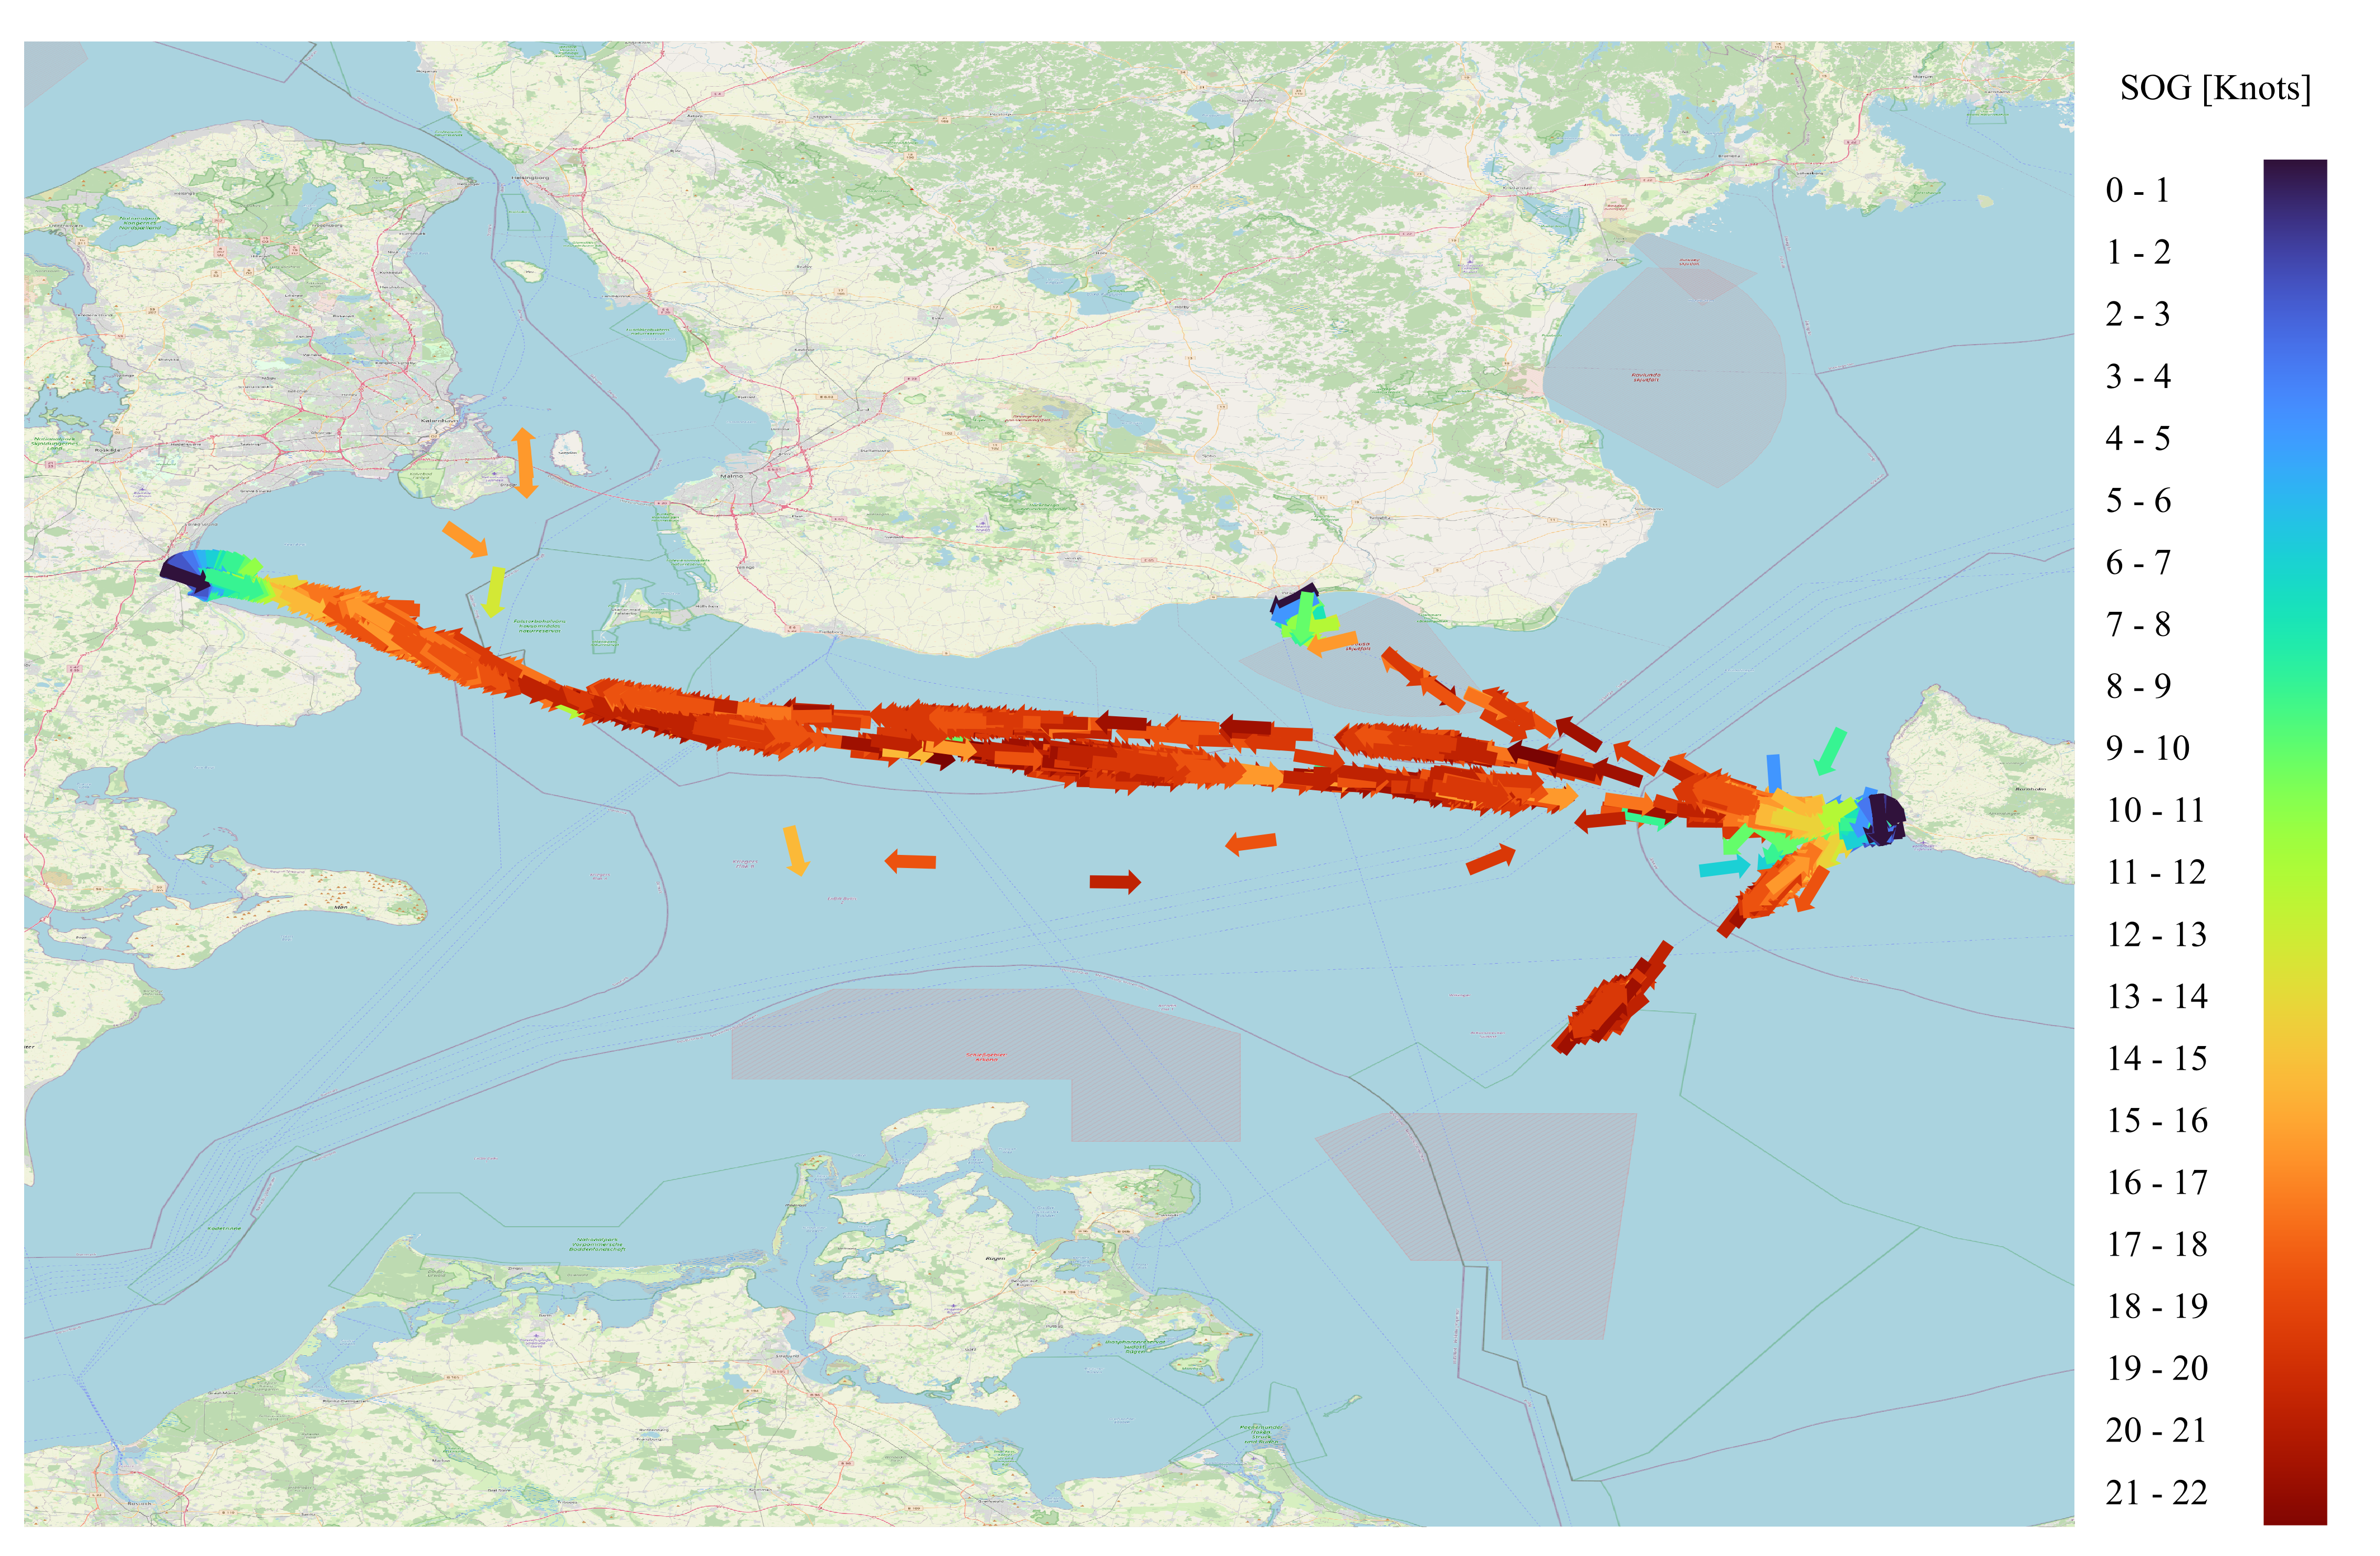
\includegraphics[width=0.8\textwidth]{02_figures/SassnitznoFilter.png}
%         \caption{Journey of the ship in a year}
%         \label{fig:YearJourney}
% \end{figure}

From preliminary analysis, possible source of error is identified for data points representing current speed. In range of current speed between $0.01$ and $0.03$ [m/s], noticeable peak in data points is observed as shown in \Cref{fig:anomalies_sog_curspeed}. This peak attributed to missing information on northward and eastward current speed in some data points from the provided dataset. This resulted in single random error value for current speed which resulted in the peak observed in the histogram.\\ 

\begin{figure}[h]
    \centering
        \includegraphics[width=0.9\textwidth]{02_figures/sog_curspeed_anomalies.png}
        \caption{Histogram plot of pre-filtered SOG and current speed}
        \label{fig:anomalies_sog_curspeed}
\end{figure}

To address the missing values, the missing values for eastward current and northward current are imputed using {\tt KNNImputer} feature from \scikit/. This is necessary as modelling package by \scikit/ cannot handle missing values. During imputing, each sample's missing values are imputed using the mean of nearest neighbour found in training dataset \bcitep{FabianPedregosa.2011}. Imputing strategy using k-nearest neighbour is considered as it should reflect the weather conditions within the region of missing values. Once the missing values of northward and southward current are imputed, the current speed for the missing values will be recalculated. The imputing approach using k-nearest neighbour is also applied to other weather features that contained missing values i.e. {\tt NaN} values.\\

\subsection{Feature Selection}\label{sec:feature_select}

To select appropriate features for the model, correlation between the features is first studied. Feature selection is necessary to simplify the model and subsequently save computing cost during training. Selection of features is based on statistical approach of High Correlation Filter proposed by Abebe et al. \bcitep{Abebe.2020}. This approach considers pairs of features with correlation features higher than 0.7 as one entity. However, the selection of highly correlated features must not violate physical knowledge. Therefore, the feature selection in this study is based on physical justification and this takes priority over purely statistical reasoning.\\

From AIS data, the information on \emph{time, latitude, longitude, width and length} are not included for training. Time, latitude and longitude only describe the location of the ship at a particular position and the width and length of ship are constant dimensions. As discussed in \Cref{sec:weather_definition}, the features \emph{combined wind wave swell height, swell height, maximum wave height and wind wave height} are physically correlated. The combined wind wave swell height defines the significant wave height $H_{1/3}$ and can be described using \Cref{eqn:H_sig_root}, \Cref{eqn:H_s_and_Tp} shows that the significant wave height also can be used to identify weather the sea is swell or wind sea dominated.\\

With that, it is clear that significant wave height should be retained for modelling, as many wave properties can be derived from it. The features swell height, wind wave height and maximum wave height will be dropped as it can be defined through significant wave height $H_{1/3}$. This decision is also statistically supported through the high correlation filter method. As shown in \Cref{fig:heatmap1}, high correlation are obtained between the $H_{1/3}$, swell height, wind wave height and maximum wave height.\\

\begin{figure}[ht]
    \centering
    \includegraphics[width=.9\linewidth,height=.9\textheight,keepaspectratio]{02_figures/heatmap_corr_ovr.png}
    \caption{Correlation Heat Map}
    \label{fig:heatmap_ovr}
\end{figure}

From \Cref{fig:heatmap1}, high correlation is observed between wave period, swell period and wind wave period. As discussed in \Cref{sec:weather_definition}, the sea state can be described through the significant height $H_{1/3}$ and spectral peak $T_p$ with help of Torsethaugen peak \bcitep{K.Torsethaugen.2004}. Hence, the features swell period and wind wave period are discarded as it only distinguish whether the sea is dominated by swell or by wind. The feature wave period will still be retained. As a result, the features ``true wind wave direction'' and ``true swell direction'' will be excluded from consideration since the features that account for their magnitude have been discarded.\\

Statistically, the heading and COG are highly correlated, but both features are retained as it explain two different parameters of the ship. Course Over Ground reflects the ship course heading while heading represented the actual heading of the ship at a particular point of time. Same principle also apply between air temperature above ocean and sea surface temperature. Air temperature above oceans represents the temperature of wind while sea surface temperature represents current temperature of current.\\

From feature selection, 5 features from AIS data are discarded while 11 features are removed from the weather data. To predict the ship speed, The SOG will be selected as the label to train the model. The remaining attributes will be selected as training features. This is summarised in \Cref{tbl:dataset_train_struct}.
\begin{table}
    \footnotesize
    \centering
    % \resizebox {\textwidth}{!}
    {\begin{tabular}{ p{8cm}c }
    \hline
    \multicolumn{2}{l}{\textbf{Training Label}}\\
    \hline
    SOG [Knots] & {\tt sog} \\
    \hline
    \multicolumn{2}{l}{\textbf{Training Features}}\\
    \hline
    COG [m/s] & {\tt cog}  \\
    Heading [°] & {\tt heading}  \\
    Draught [m] & {\tt draught} \\
    Wind Speed [m/s] & {\tt windspeed} \\
    Air Temperature Above Oceans [K] & {\tt oceantemperature} \\
    Maximum Wave Height [m] & {\tt waveheight} \\
    Wave Period [s] & {\tt waveperiod}\\
    Sea Surface Temperature [K] & {\tt surftemp}\\
    Combined Wind Wave Swell Height [m] &  {\tt windwaveswellheight} \\
    Current Speed [m/s] & {\tt curspeed} \\
    True Wind Direction [°] & {\tt truewinddir}  \\
    True Current Direction [°] & {\tt truecurrentdir} \\
    True Wave Direction [°] & {\tt truewavedir} \\
    \hline
    \end{tabular}}
\caption{Structure of fused dataset}\label{tbl:dataset_train_struct}
\end{table}

\section{Modelling}\label{sec:modelling}

In this section, the modelling of ship speed through SOG using selected features will be performed using tree-based regressor model. The tree-based regressor model considered are decision tree regressor, random forest regressor and extra-tree regressor. In addition, the tree-based models are compared against multiple linear regressor for benchmarking. For training, the dataset is split into training, validation and test dataset in ratio of 73:18:9. Journey data from the month of June is arbitrarily selected as test dataset. The remaining dataset will be split into training and validation dataset in 80:20 ratio. The trained model will be evaluated using k-fold cross validation, if the best model is not obtained, then the parameter of the tree-based regressor will be tuned until no further improvements of the model can be made.\\


\subsection{Performance Metrics for Validation}\label{sec:perf_metrics}

To gain sensible estimate of model performance and how precise a model is, the model will be cross validated by means of k-folding. K-fold cross validation split the training set into k subsets which is called \emph{folds}, then the model will be trained k times using k-1 subsets and remaining one for validation, this process is illustrated in \Cref{fig:kfold}. For each iteration, each model is evaluated using different performance metrics such as \textbf{Coefficient of Determination ($R^2$), Explained Variance (EV), Mean Absolute Error (MAE),Root Mean Square (RMSE), Median Absolute Deviation (MAD) and Mean Absolute Percentage Error (MAPE)}. The results from each iteration is then averaged, where the information on model precision can be gained from the standard deviation. Performing k-fold cross validation checks model robustness against different datasets. The properties of each performance metric will be discussed in the following sections.

\begin{figure}
    \centering
    \includegraphics[width=.85\textwidth]{02_figures/kfold.png}
    \caption{Visual illustration of k-folding, Grey shaded box represents the validation data while white box represents the training data}
    \label{fig:kfold}
\end{figure}

\subsubsection*{Coefficient of Determination ({$R^2$})}\label{sec:rsquared}

The coefficient of determination $R^2$ gives a measure on prediction quality, $R^2$ quantifies the ability of the regression model to approximate the actual values. $R^2 $ is defined by \Cref{eqn:rsquared}, where $y$ represents true target output, $\hat{y}$ represents the predictor output and $\overline{y}$ represents the mean. $R^2$ score range between 0 and 1, higher values i.e. $R^2 \rightarrow 1$ indicate better model fit and score of 1 indicate perfect prediction.\\

\begin{equation}\label{eqn:rsquared}
    R^2(y,\hat{y}) = 1 - \frac{\sum_{i = 1}^{n} (y_{\text{i}} - \hat{y}_{\text{i}} )^2 }{\sum_{i = 1}^{n} (y_{\text{i}} - \overline{y}_{\text{i}})^2} \quad \textbf{where} \quad \overline{y} = \frac{1}{n}\sum_{1}^{n} y_\text{i}
\end{equation}

\subsubsection*{Explained Variance (EV)}\label{sec:expVar}

Explained variance indicate how well a model can capture variance from a dataset. It is defined by \Cref{eqn:expVar}, where $\sigma_x$ represents standard deviation of parameter $x$. EV score range between 0 and 1, where the best score of $EV = 1$ can be obtained if $\sigma^2_{(y-\hat{y})} \rightarrow 0$.\\  

\begin{equation}\label{eqn:expVar}
    EV(y,\hat{y}) = 1 - \frac{\sigma^2_{(y-\hat{y})}}{\sigma^2_{y}}
\end{equation}

\subsubsection*{Mean Absolute Error (MAE)}\label{sec:MAE}

MAE indicated the expected value of absolute ($L^1$ norm) error, and it can be calculated by:

\begin{equation}\label{eqn:MAE}
    MAE(y,\hat{y}) = \frac{1}{n}\sum_{i=1}^{n} |y_{\text{i}} - \hat{y}_{\text{i}}| 
\end{equation}

\subsubsection*{Root Mean Square Error (RMSE)}\label{sec:RMSE}

The RMSE describe the expected value of quadratic error. RMSE place large penalty on large deviation between true and estimated values and for this reason, it can be used to as a metric to indicate model performance against outliers. Ideal score is observed when $\text{RMSE} \rightarrow 0$. RMSE can be considered as absolute measure of model fitness. Omitting the root term, RMSE becomes MSE, which is the loss function of \Cref{eqn:costfun} that is used to determine the most optimal split in a regression decision tree.\\

\begin{equation}\label{eqn:RMSE}
    RMSE(y,\hat{y}) = \sqrt{\frac{1}{n}\sum_{i=1}^{n} (y_{\text{i}} - \hat{y}_{\text{i}})^2} 
\end{equation}

\subsubsection*{Median Absolute Deviation (MAD)}\label{sec:MAD} 

MAD is a performance metrics that considers the median of the absolute errors. It is robust to outlier as it only consider median performance

\begin{equation}\label{eqn:MAD}
    MAD(y,\hat{y}) =  \text{median} (|y_{\text{1}} - \hat{y}_{\text{1}}|,\dots,|y_{\text{i}} - \hat{y}_{\text{i}}|)
\end{equation}

\subsubsection*{Mean Absolute Percentage Error (MAPE)}

Is an alternative to MAE, which provide easier interpretation, the result of MAPE can be interpreted according to \Cref{eqn:MAPE} \bcitep{MontanoMoreno.2013}. The usage of MAPE in model evaluation is to get initial estimate, as MAPE comes with some drawback such as instability when $y_i = 0$ and it may lead to biased forecast \bcitep{Gkerekos.2019}. As such, the evaluation of the model performance will be mainly based on MAE and RMSE.    

\begin{equation}\label{eqn:MAPE}
    MAPE(y,\hat{y}) = \frac{1}{n}\sum_{i=1}^{n} \biggl|\frac{y_{\text{i}} - \hat{y}_{\text{i}}}{y_i}\biggr| \cdot 100\%  \quad \textbf{with} \quad \begin{array}{l c}
        \text{MAPE} & \text{Interpretation}\\
        \hline\\
        < 10 & \text{Highly accurate forecasting} \\
        10-20 & \text{Good Forecasting} \\
        20-50 & \text{Reasonable forecasting}\\
        > 50 & \text{Inaccurate forecasting} \\
    \end{array}
\end{equation}

\subsection{Model Hyperparameter Optimisation}\label{sec:hpo}

The subject of parameter tuning was briefly discussed in \Cref{sec:dt_theo}. In \Cref{sec:dt_theo} parameter tuning was applied to decision tree regressor to avoid overfitting by changing the minimum amount of samples a leaf node has. This example implies that altering model hyperparameter will affect the model performance. However, the optimisation of the hyperparameter cannot be performed \emph{a priori} and as such iterative process will be performed until best hyperparameter value is found.\\ 

% \begin{table}[ht]
%     \scriptsize
%     \centering
%     % \resizebox {\textwidth}{!}
%     {\begin{tabular}{ p{0.33\textwidth}p{3cm}p{3cm}p{3cm}  }
%     \hline
%     \multicolumn{1}{c}{\textbf{Model}} & \multicolumn{1}{c}{\textbf{Decision Tree}}  & \multicolumn{1}{c} {\textbf{Random Forest}} & \multicolumn{1}{c}{\textbf{Extra-Trees}}\\
%     \hline
%     Number of trees & \multicolumn{1}{c}{1} & \multicolumn{1}{c}{Many} & \multicolumn{1}{c}{Many}\\
%     Features considered for split at each node &   \multicolumn{1}{c}{All features}  & \multicolumn{1}{c}{Random subset of features} & \multicolumn{1}{c}{Random subset of features} \\
%     Bootstrapping & \multicolumn{1}{c}{Not applied} & \multicolumn{1}{c}{Yes} & \multicolumn{1}{c}{No}\\
%     Split Rule  & \multicolumn{1}{c}{Best split} & \multicolumn{1}{c}{Best split}& \multicolumn{1}{c}{Random split}\\
%     \end{tabular}}
% \caption{Comparison of tree based model from \Cref{sec:tree_intro}}\label{tbl:table_trees}
% \end{table}

\scikit/ offers {\tt GridSearchCV} and {\tt RandomizedSearchCV} to help search for the most optimal hyperparameter. Both solutions operate with similar principle: The selected hyperparameters to be tuned with its value range is evaluated using cross validation to evaluate the best possible combination between the selected hyperparameters. The difference between {\tt GridSearchCV} and {\tt RandomizedSearchCV} lies in how it searches for the best value for the selected hyperparameters: {\tt GridSearchCV} involves construction of grids containing all possible combinations of hyperparameter value in specified range.{\tt RandomizedSearchCV} randomly samples hyperparameter values.\\ 

The exhaustive nature of {\tt GridSearchCV} means that it is computationally costly to perform, especially when there are multiple hyperparameters to be considered and value search space is large. {\tt RandomizedSearchCV} gives more control to computing budget by setting the number of iteration and usually produces more accurate results than {\tt GridSearchCV} approach. \bcitep{Geron.2019,J.Bergstra.2012}. \\

For this reason, the {\tt RandomizedSearchCV} will be employed to search for best possible hyperparameter. However, the limitation of \emph{a priori} knowledge of hyperparameter value still exists. In spite of {\tt RandomizedSearchCV} ability to control the computational budget, it is still takes considerable time to obtain the best hyperparameter value. The computational budget may be spent on searches in unpromising search space. With that, initial exploration on the effect of each hyperparameter on model performance will be performed to give better overview on which search space that should be considered during hyperparameter optimisation. In the next subsections, the effect of tunable hyperparameter of tree-based model from \scikit/ will be explored to give baseline numbers for the search space. RMSE is used as performance metrics as the hyperparameter parameter optimisation done in this thesis aims to reduce the error during prediction. \\ 

\subsubsection*{Number of features}\label{sec:max_features}

Defined with default value as {\tt max\_features=None} in \scikit/. This hyperparameter controls the number of features to be considered when looking for the best split, the default {\tt None} option means it will consider all features. This parameter tuning is available for Decision Tree Regressor, Random Forest Regressor and Extra-Tree Regressor. Initial exploration indicated Random Forest Regressor and Extra Tree Regressor benefit from considering more features, Decision Tree Regressor requires further fine-tuning to optimise the model as the default {\tt None} means it will consider all features when searching for best split.\\ 

\begin{figure}[h]
    \centering
        \includegraphics[width=.85\textwidth]{02_figures/hpo_n_features.png}
        \caption{Hyperparameter tuning of {\tt max\_features}}
        \label{fig:hpo_n_features}
\end{figure}

\subsubsection*{Number of sample in a leaf node}\label{sec:min_samples_leaf}

Defined with default value as {\tt min\_samples\_leaf=1} in \scikit/. This parameter controls number of samples required to be at leaf node, where split point will be considered if the leaf contains at least {\tt min\_samples\_leaf=n} training samples in each left and right branch. As shown in \Cref{fig:geron6_6}, tuning this hyperparameter to higher values helps to smoothen the model and avoid overfitting. However, this may lead to underfitting as the model is unable to capture the trend within the data. This is supported by the findings shown in \Cref{fig:hpo_min_samples_leaf}, the DTR benefits from regularisation at certain breakeven point, in this case, it is found to be at {\tt min\_samples\_leaf=4}. But after this breakeven point, the model's performance degrades. It is also observed that RFR and ETR does not benefit from any form of regularisation.  

\begin{figure}[h]
    \centering
        \includegraphics[width=.85\textwidth]{02_figures/hpo_min_samples_leaf.png}
        \caption{Hyperparameter tuning of {\tt min\_samples\_leaf}}
        \label{fig:hpo_min_samples_leaf}
\end{figure}

\subsubsection*{Depth of Tree}\label{sec:max_depth}

Defined with default value as {\tt max\_depth=None} in \scikit/. This hyperparameter controls the growth of the tree. Leaving it at {\tt max\_depth=None} means the tree will grow until all leaves are pure i.e. until minimum MSE is obtained or when the number of samples is less than the minimum number of samples required to split an internal node. Similar to {\tt min\_samples\_leaf}, DTR shows improvement until a certain breakeven point. RFR performance seems to stabilise at certain depth while ETR benefits from allowing full growth of the tree. The results are summarised in \Cref{fig:hpo_max_depth}  

\begin{figure}[h]
    \centering
        \includegraphics[width=.95\textwidth]{02_figures/hpo_max_depth.png}
        \caption{Hyperparameter tuning of {\tt max\_depth}}
        \label{fig:hpo_max_depth}
\end{figure}

\subsubsection*{Number of Trees}\label{sec:n_estimators}

Defined with default value as {\tt n\_estimators=100}. This hyperparameter controls the amount of trees i.e. predictors in a forest. Tuning of number of trees will have an effect on the training time and it is only available to RFR and ETR. The default value seems to yield satisfactory result, as the performance for both RFR and ETR stabilise after in this case stabilise after 100 trees, as seen in \Cref{fig:hpo_n_features}. 

\begin{figure}[h]
    \centering
        \includegraphics[width=.95\textwidth]{02_figures/hpo_n_estimators.png}
        \caption{Hyperparameter tuning of {\tt n\_estimators}}
        \label{fig:n_estimators}
\end{figure}


\begin{figure}
    \centering
        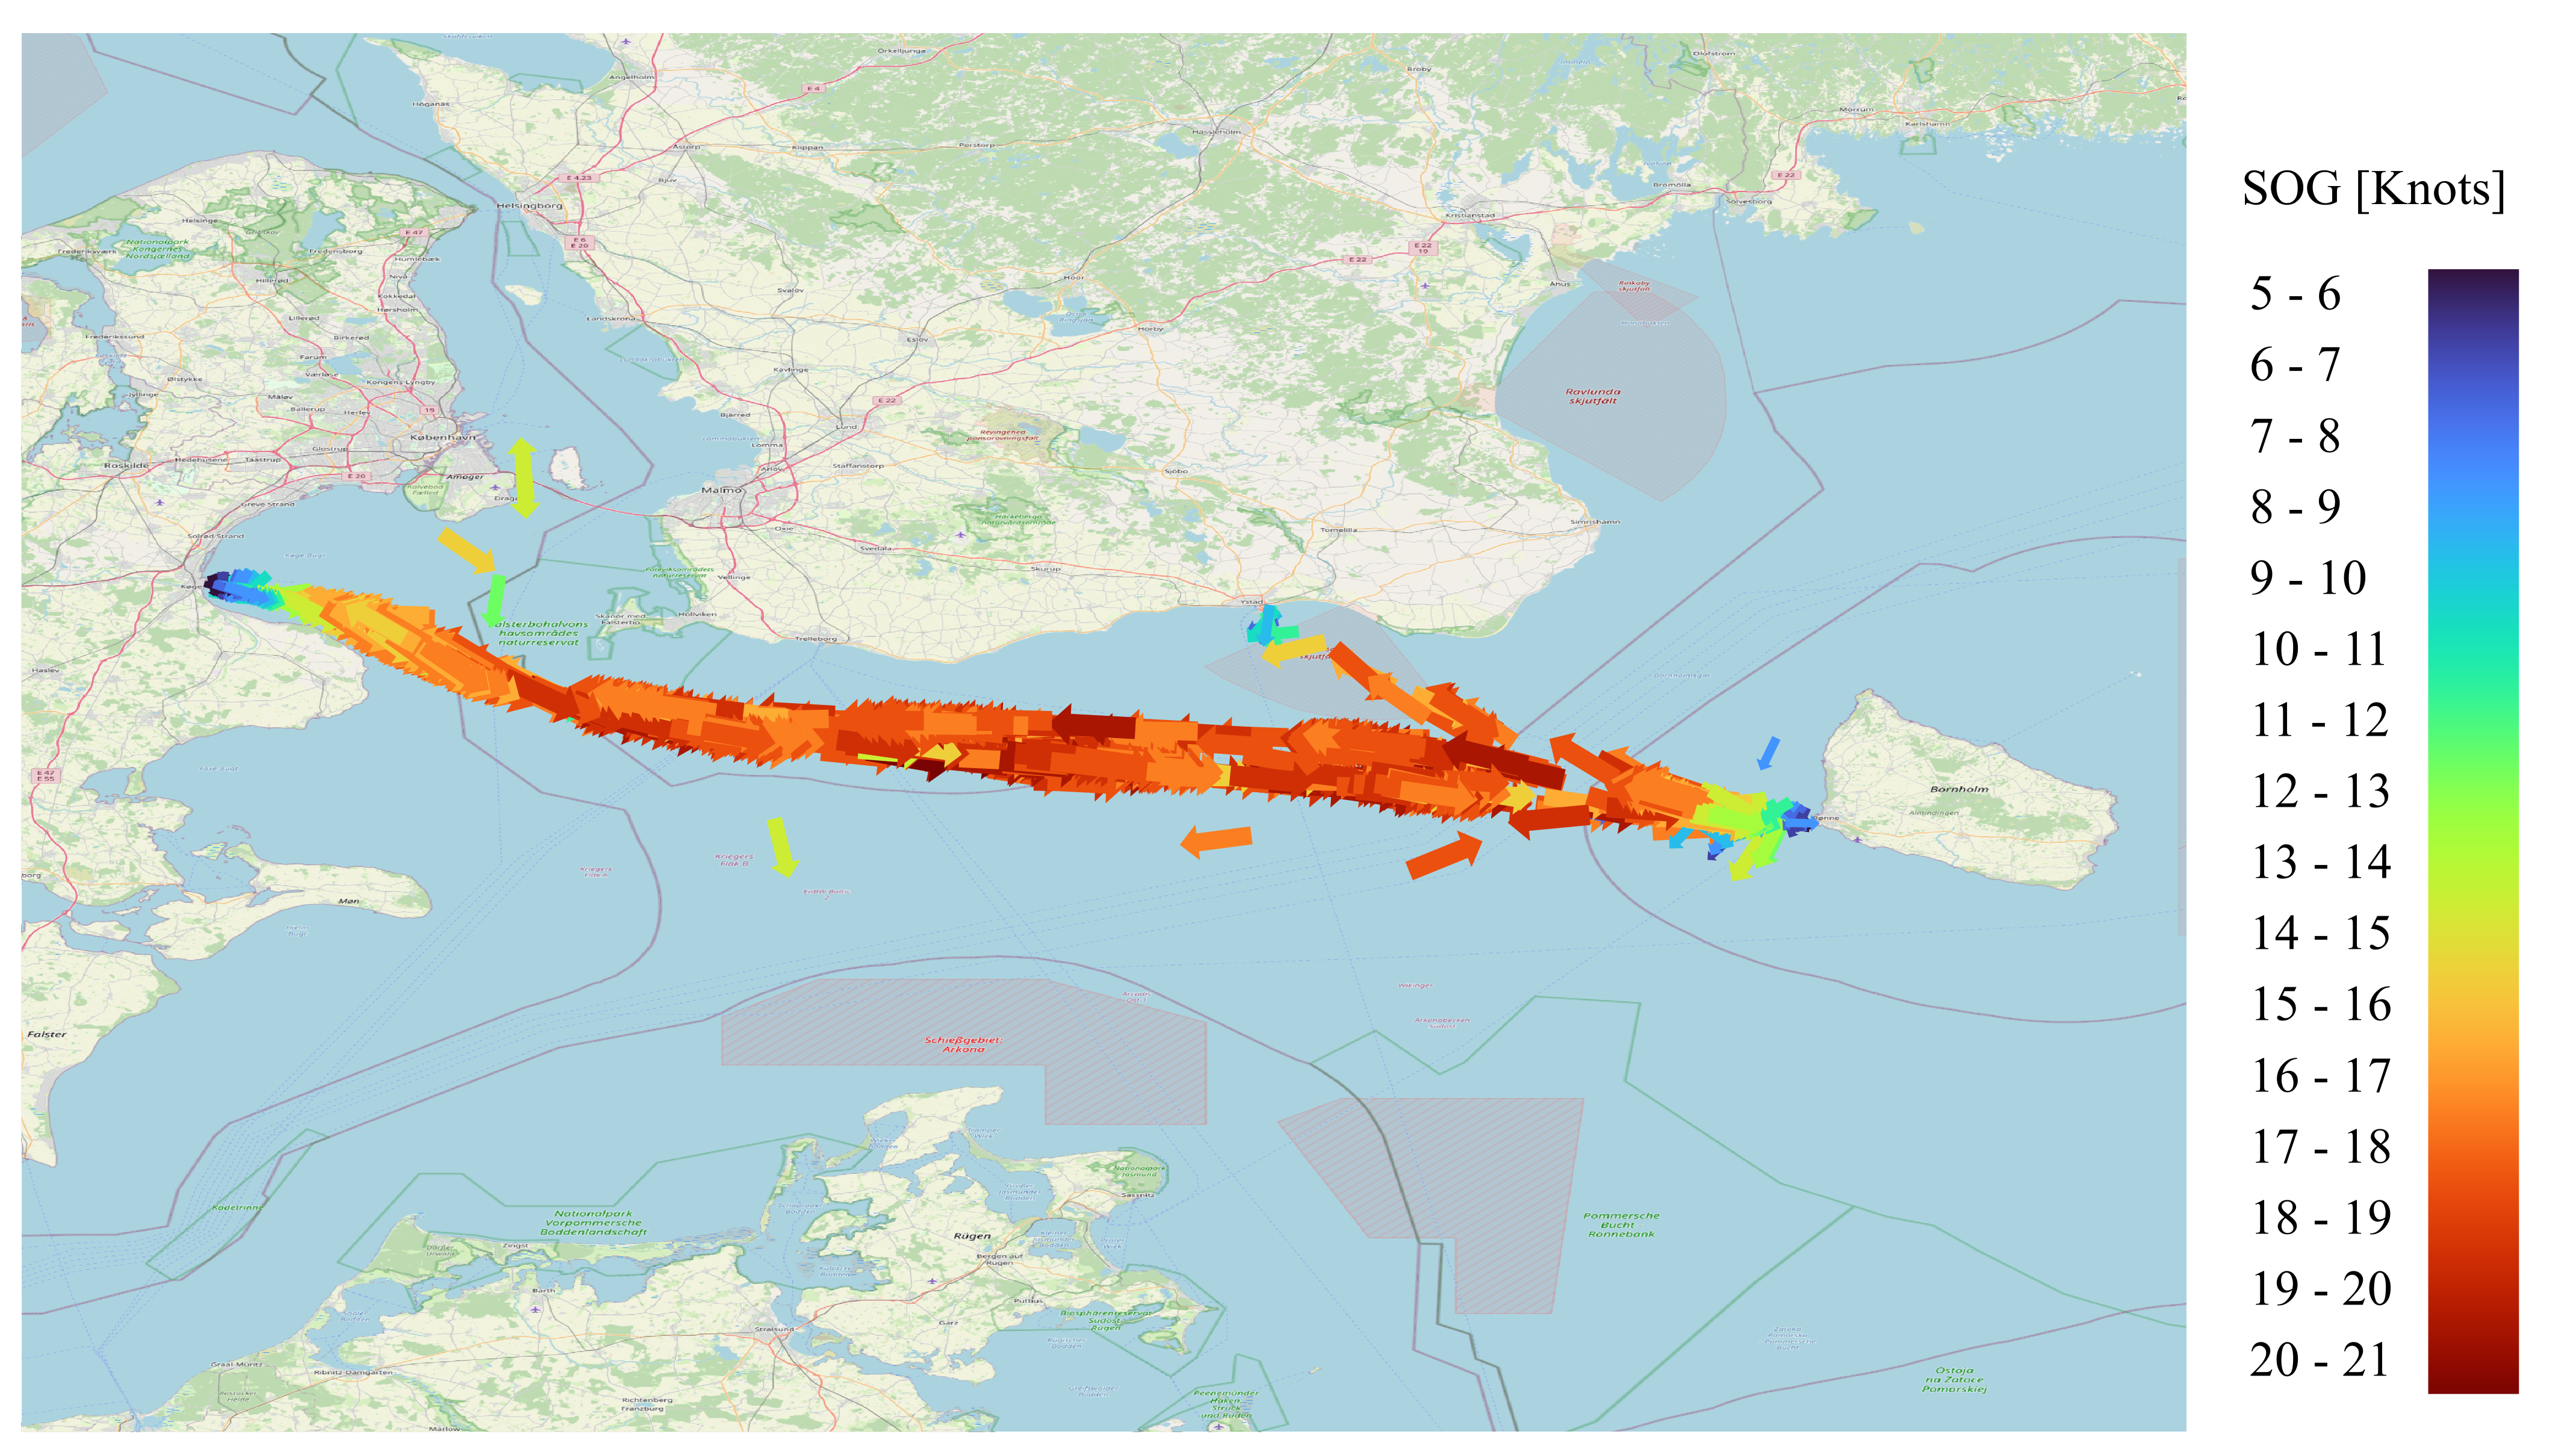
\includegraphics[width=.85\textwidth]{02_figures/JuneFilter.png}
        \caption{Journey of the ship in June}
        \label{fig:JuneJourney}
\end{figure}

\subsection{Methodology Application}\label{sec:methodology_application}

As such, this thesis aims to find optimisation possibilities for the BBM to extract maximum prediction performance from tree-based model. The estimation of engine power using Holtrop-Mennen method involves a lot of The approximations. To ensure correctness during estimation of engine power, the approximations are based on   of ship dimensions and mechanical data are based  

\begin{itemize}
    \item Two data sources are imported. {\tt AIS\_weather\_H\_ok2\_copy.csv} \\ and {\tt AIS\_weather\_h\_rename\_copy.csv}. The information from the latter comma delimited 
    file will be used for calculating the ship Speed Through Water (STW).  
    The information required is the true north current direction. Which is obtained from the vector component of the Northward and Southward current.
    \item This dataframe will be merged with the main dataframe from \\ the file {\tt AIS\_weather\_H\_ok2\_copy.csv}.
    \item Omission of the journey data between Ronne and Sassnitz
    \item SOG threshold is applied to omit ship mooring and maneuvering to accurately represent the ship's steady state operation 
    \cite{Abebe.2020,BalBesikci.2016,Gkerekos.2019,Yang.2020}. This threshold is selected as 5 knots according to \cite{Abebe.2020}
    \item The AIS data from June is filtered. This data will be used as validation data to check the model's performance.
\end{itemize}
 
\subsection{Data Analysis}
\begin{itemize}
    \item The features are represented in a histogram plot. For the feature Current speed, anomaly is detected. Certain spike is detected around $0.01 - 0.03$ \verb|m/s|. Reasons unknown. The data is retained, including the spike, until a definitive answer can be found.
    \item OPEN QUESTION : What is the necessity of feature standardization / normalization ? Normalization is required for ANN as model training requires the value between 0 and 1. But in case of RFR, there is no such requirement. Through testing, data standardization also does not seem to improve the model's performance. 
\end{itemize}




\begin{sidewaysfigure}
    \includegraphics[width=\linewidth,height=\textheight,keepaspectratio]{02_figures/outputhist.png}
    \caption{Histogram of the features}
    \label{sidewaysfig:hist1}
\end{sidewaysfigure}

\newpage

\begin{itemize}
    \item The correlation of the features against SOG are determined. It is found that :
    \begin{itemize}
        \item Draught
        \item Course Over Ground (COG)
        \item heading
        \item Wind Speed
        \item Current Speed
        \item True Current direction
    \end{itemize}
    Have relatively stronger correlation to SOG compared to other features, albeit the correlation is a weak one
    \item The correlation between the features is displayed using the following the heat map. From the heat map it can be observed that between these features:
    \begin{itemize}
        \item Waveheight and wind wave swell height
        \item Waveheight and wind wave height
        \item Windwaveswellheight and wave period
    \end{itemize}
    Have a strong correlation between each other.  
    \item Open topic: 
    \begin{itemize}
        \item Feature reduction is possible, \cite{Abebe.2020} suggested high feature correlation filter, the filter suggest that two features which has a high correlation $(>90\%)$ is to be combined into a single feature. But the author is unsure whether this combination is physically sensible. Hence, this filter is yet to be applied for feature reduction. 
        \item Some of these features can be connected through wave equations, but the author has not found an equation which could relate these features.
    \end{itemize}
    \item The random forest regressor could not function when \verb|NaN| values are present. With that, the missing values are filled in using the {\tt imputer} function. The missing values are filled in by means of \verb|KNN|.
\end{itemize}

\newpage

\begin{figure}[h]
    \includegraphics[width=\linewidth,height=\textheight,keepaspectratio]{02_figures/heatmap_corr.png}
    \caption{Correlation Heat Map}
    \label{fig:heatmap1}
\end{figure}

\subsection{Modelling}

\begin{itemize}
    \item The data is split into 80:20 ratio. But considering the validation data, it is split into approximately 73:18:9.
    \item The model is then trained using Random Forest Regression (RFR). Additional training is also performed using Decision Tree Regressor (DTR). DTR model performance will be used as a benchmark as it is also a tree-based modelling method with similar methodology to RFR.
    \item The computational time of DTR is significantly faster than RFR
    Model Evaluation    
\end{itemize}

\subsection{Predicting STW}
\begin{itemize}
    \item The ship's Speed Through Water STW can be calculated using vector component of the SOG and current speed. The direction used will be according to True North. \cite{Yang.2020,Zhou.2020}
    \item SOG represents the speed of the ship with reference to the ground, while the STW represent the ship's speed with reference to water.
    \item SOG also can be termed by the ship's speed that is captured by the GPS, and does not consider any effect of the current
    \item This means that the ship's STW will be greater than the ship's SOG when there is current moving against the ship's movement direction and vice versa 
    \item The vector decomposition can be defined from the following equations, which is based on the equation by \cite{Yang.2020}:
    \begin{itemize}
        \item The ship's SOG $V_g$ can be decomposed into $V_{g}^x$ and $V_{g}^y$, which represents the $x$ and $y$ components of the SOG respectively using the ship's course heading (COG) $\beta$ \emph{with respect to True North}:
        \begin{equation}\label{eqvgx}
            V_{g}^x = V_g\sin(\beta)   
        \end{equation}
        \begin{equation}\label{eqvgy}
            V_{g}^y = V_g\cos(\beta)   
        \end{equation}
        \item To consider the effect of sea current. The current speed $V_c$ will also be decomposed to $x$ and $y$ components respectively using the current direction $\gamma$ \emph{with respect to True North}:
        \begin{equation}\label{eqvcx}
            V_{c}^x = V_g\sin(\gamma)   
        \end{equation}
        \begin{equation}\label{eqvcy}
            V_{c}^y = V_g\cos(\gamma)   
        \end{equation}
        \item from here the ship' STW $V_{wx}$ and $V_{wy}$ component can be found from the following equation: 
        \begin{equation}
            V_{w}^x = V_{g}^x - V_{c}^x    
        \end{equation}
        \begin{equation}
            V_{w}^y = V_{g}^y - V_{c}^y 
        \end{equation}
        \item The magnitude of the STW can be readily obtained from the following vector synthesis
        \begin{equation}
            V_w = \sqrt{(V_{w}^x)^2 + (V_{w}^y)^2} 
        \end{equation}
    \end{itemize}
    \newpage

    \item This principle is applied to the following Python script. \ref{eqvcx}

\begin{python}
       
        # Convert SOG from [Knots] to [m/s]
    
        dfprog["vgms"] = dfprog["sog_pred"]/1.9438
        
        # Convert the angles from [Degrees] to [Radians]

        rad_gamma = np.deg2rad(dfprog["gamma"])
        rad_cog = np.deg2rad(dfprog["cog"])

        # Decomposition in x-component

        dfprog["vgx"] = dfprog["vgms"] * np.sin(rad_cog)
        dfprog["vcx"] = dfprog["curspeed"] * np.sin(rad_gamma)
        dfprog["stw_x"] = (dfprog["vgx"] - dfprog["vcx"])

        # Decomposition in y-component

        dfprog["vgy"] = dfprog["vgms"] * np.cos(rad_cog)
        dfprog["vcy"] = dfprog["curspeed"] * np.cos(rad_gamma)
        dfprog["stw_y"] = (dfprog["vgy"] - dfprog["vcy"])

        # Vector synthesis and reconversion to [Knots] from [m/s]

        dfprog["vwms_p"] = np.sqrt(dfprog["stw_x"]**2 + dfprog["stw_y"]**2)
        dfprog["stw_pred"] = dfprog["vwms_p"]*1.9438  

    \end{python}
\newpage

\begin{sidewaysfigure}
    \includegraphics[width=\linewidth,height=\textheight,keepaspectratio]{02_figures/rfrftree.png}
    \caption{Correlation Heat Map}
    \label{fig:Random Forest Regression Tree}
\end{sidewaysfigure}


\end{itemize}


\newpage
\chapter{Result and Discussion} \label{chp:result_and_discussion}

The performance of GBM will be evaluated by means of a case study using the test dataset. The test dataset comprises journey data from the whole year of 2021. The first part will focus on performance evaluation of BBM, where the trained model will be used to predict the SOG. The second part focus on the power estimation method using Holtrop-Mennen method. The output of BBM, which is the ship SOG, will be fed to the WBM to estimate the power. For further clarity regarding the methodology, the following steps are taken which are based on the proposed methodology shown in \Cref{fig:flowchart_BBM} and \Cref{fig:flowchart_WBM}. For generation of the BBM, the steps taken are:

\begin{enumerate}
    \setlength\itemsep{0em}
    \item Dataset is loaded.
    \item Identify and remove any anomalies.
    \item Remove static and unneeded features.
    \item Apply speed threshold of 5 knots.
    \item Highly correlated features are combined/removed based on physical and statistical reasoning.
    \item Impute missing values using {\tt KNNImputer}.
    \item Split the dataset into training and testing.
    \item Train the model using the whole dataset with default hyperparameter.
    \item Evaluate model performance using k-fold cross-validation.
    \item Tune the model until the best model is obtained.
    \item For the case study, the best models will be used to predict the SOG using the test dataset.
\end{enumerate}

Subsequently, for FOC calculation, the following steps are taken:

\begin{enumerate}
    \setlength\itemsep{0em}
    \item The test dataset is split into seasonal data. Summer-Fall season and Winter-Spring season which correspond to data for 6 months respectively.
    \item Impute missing values using {\tt KNNImputer}.
    \item SOG is converted to STW.
    \item Calculate calm water resistance $R_{CALM}$.
    \item Calculate added resistance due to wave $R_{AW}$.
    \item Calculate added resistance due to wind $R_{AA}$.
    \item Calculate total effective power $P_E$ using total resistance $R_{TOTAL}$.
    \item Calculate brake power $P_B$ from total efficiencies.
    \item Plot resulting regression line for Power-Speed curve from all models and actual case. 
    \item Calculate the FOC by considering the engine SFOC and operation time.
    \item Plot resulting regression line for FOC-Speed curve from all models and actual case.
    \item Evaluate the performance of the model generated from the regression lines.
\end{enumerate}

\section{Evaluation of BBM}\label{sec:BBM_tree_evaluate}

\subsection*{Model Training and Selection of Optimal Parameter}\label{sec:hpo_select_train}

As mentioned in \Cref{sec:BBM_modelling}. There are 2871 data points available for training. To help narrow the search range of the hyperparameters for the tree-based model, RMSE plots against different values of hyperparameters will be performed. This method was presented in \Cref{sec:hpo}. The hyperparameter will be iteratively tuned until the best model is obtained. The result of the optimal parameter is found in \Cref{tbl:hpo_optimal}. The model training is executed using \textbf{AMD Ryzen 7 2700X, Eight-Core Processor $@$ 3.7 GHz processor with 16384 MB installed RAM}.\\


\begin{table}[ht]
    \footnotesize
    \centering
    % \resizebox {\textwidth}{!}
    {\begin{tabular}{ p{0.1\linewidth} p{0.2\linewidth} p{0.3\linewidth}}
    \hline
    Model & Training time [s] & Optimal Hyperparameter \\
    \hline
    DTR & 0.044 & None \\
    $\text{DTR}_{OPT}$ & 0.021  & {\tt min\_samples\_split = 7}\\
    &&{\tt min\_samples\_leaf = 10}\\
    &&{\tt max\_features = 12}\\
    &&{\tt max\_depth = 8}\\
    RFR & 4.112 & None \\
    $\text{RFR}_{OPT}$ & 3.431  & {\tt min\_samples\_split = 2}\\
    &&{\tt min\_samples\_leaf = 1}\\
    &&{\tt max\_features = 10}\\
    &&{\tt max\_depth = 120}\\
    &&{\tt n\_estimators = 100}\\
    ETR & 0.944 & None \\
    $\text{ETR}_{OPT}$ & 4.390  & {\tt min\_samples\_split = 9}\\
    &&{\tt min\_samples\_leaf = 1}\\
    &&{\tt max\_features = 12}\\
    &&{\tt max\_depth = 120}\\
    &&{\tt n\_estimators = 800}\\
    MLR & 0.004  & None\\
    \hline
    \end{tabular}}
\caption{Optimal hyperparameter with training time of each model}\label{tbl:hpo_optimal}
\end{table}

With the default hyperparameter, RFR takes the longest training time followed by ETR and DTR. This is expected as RFR uses greedy algorithm i.e. it looks for the best possible feature when splitting the node. ETR takes significantly shorter time to train as ETR randomly select for features when splitting the node. DTR takes the shortest training time as it only generates a single tree. However, in the case of optimised model, ETR takes a longer time to train compared to RFR. This is caused by the number of trees in the optimised model which is controlled by the parameter {\tt n\_estimator}, the optimised ETR model has 800 trees in comparison to 100 trees of RFR. It is also observed that the training time of optimised DTR model is halved as pruning the tree resulted in a simpler model to train. \\

To further investigate the effect of hyperparameter optimisation, the learning curve of each tree-based model is plotted. For DTR, generated model with default parameter will result in a model that heavily overfits the training data, which is evident from the large gap between the training error and validation error which indicated a high variance as shown in \Cref{fig:learn_curve_DTR_RMSE}. Regularisation i.e. parameter tuning of the DTR model helps balance between bias and variance by trading bias for variance. This is observed from the substantial reduction in the gap between the training and validation error from \Cref{fig:learn_curve_DTR_RMSE}. Additionally, the learning curve indicates that the most notable improvement in model performance occurs until around 1000 data points. Beyond this point, the enhancement in model performance becomes less substantial.\\

\begin{figure}[h]
    \centering
        \includegraphics[width=.95\textwidth]{02_figures/learning_curve_dtr.png}
        \caption{Learning curve of DTR}
        \label{fig:learn_curve_DTR_RMSE}
\end{figure}

The process of hyperparameter tuning for the Random Forest Regressor (RFR) model did not show any significant improvement in model performance. This outcome aligns with the findings of  \bcitet{Kuhn.2013} and \bcitet{Hastie.2009} which was discussed in \Cref{sec:rf_theo}. The most notable improvement on model performance is observed until around 750 points, after which the model appears to reach a plateau. Furthermore, there is noticeable variance in the RFR model, which indicates that the model will have a slight tendency to overfit.\\

\begin{figure}[h]
    \centering
        \includegraphics[width=.95\textwidth]{02_figures/learning_curve_rfr_rmse.png}
        \caption{Learning curve of RFR}
        \label{fig:learn_curve_RFR_RMSE}
\end{figure}

Hyperparameter tuning helps to reduce variance in the ETR model. But it does not have any major impact on model's performance. The ETR model reaches plateau beyond 1000 data points. Suggesting that adding more data points will not result in any significant increase in model performance.\\

\begin{figure}[h]
    \centering
        \includegraphics[width=.95\textwidth]{02_figures/learning_curve_etr_rmse.png}
        \caption{Learning curve of ETR}
        \label{fig:learn_curve_ETR_RMSE}
\end{figure}

In addition to the initial exploration in \Cref{sec:hpo}, it can be concluded that hyperparameter tuning for number of features and tree depth will have the biggest impact in affecting the model's performance. To improve training time, lower number of trees should be considered for RFR and ETR model.\\


\subsection*{Analysis of trained model}\label{sec:BBM_model_eval}

\subsubsection*{Feature Importance}

As discussed in \Cref{sec:rf_theo}, tree-based models are able to quantify the impact of each feature during the split process, this is performed using {\tt feature\_importances\_} feature in \scikit/ \bcitep{Kuhn.2013}. According to documentation by \bcitet{FabianPedregosa.2011}, it is computed as the mean and the standard deviation of accumulation of the impurity decrease within each tree i.e. total reduction of the criterion brought by a feature. Alternatively, it can be defined as how much a feature is used in each tree.\\

\begin{table}[ht]
    \scriptsize
    \centering
    \resizebox {\textwidth}{!}
    {\begin{tabular}{ p{0.15\linewidth} c| p{0.15\linewidth} c| p{0.15\linewidth} c}
    \hline
    $\text{DTR}_{OPT}$ & & $\text{RFR}_{OPT}$ & & $\text{ETR}_{OPT}$\\
    \hline
    Feature & Importance & Feature & Importance & Feature & Importance\\
    \hline
    {\tt heading} & 0.6563 & {\tt heading} & 0.4927 & {\tt cog} & 0.6410 \\
    {\tt cog} & 0.3183 & {\tt cog} & 0.4183 & {\tt heading} & 0.2707 \\
    {\tt draught} & 0.0105 & {\tt draught} & 0.0210 & {\tt truecurrentdir} & 0.0200\\
    {\tt truewinddir} & 0.0047 & {\tt curspeed} & 0.0104 & {\tt draught} & 0.0144 \\
    {\tt oceantemperature} & 0.0029 & {\tt waveperiod} & 0.0093& {\tt windwaveswellheight} & 0.0112\\
    {\tt surftemp} & 0.0025&{\tt truecurrentdir} & 0.0092 & {\tt curspeed} & 0.0110\\
    {\tt waveperiod} & 0.0019 & {\tt windwaveswellheight} & 0.0084& {\tt waveperiod} & 0.0095 \\
    {\tt truecurrentdir} & 0.0010 & {\tt surftemp} & 0.0075& {\tt windspeed} & 0.0053\\
    {\tt windwaveswellheight} & 0.0008 & {\tt truewinddir} & 0.0075& {\tt surftemp} & 0.0046 \\
    {\tt curspeed} & 0.0004 & {\tt truewavedir} & 0.0058& {\tt truewavedir} & 0.0045 \\
    {\tt windspeed} & 0.0004 & {\tt oceantemperature} & 0.0057& {\tt oceantemperature} & 0.0044\\
    {\tt truwavedir} & 0.0001 & {\tt windspeed} & 0.0056& {\tt truewinddir} & 0.0033\\
    \end{tabular}}
\caption{Feature importance of different models}\label{tbl:feature_importances}
\end{table}

The feature importances for all tree-based models shown in \Cref{tbl:feature_importances} indicated that the structure of the model is significantly influenced by the features {\tt heading} and {\tt cog}. This finding indicated that the models predicted the SOG by basis of ship movement direction i.e. heading and COG for a particular location. However, in a physical sense, it will be more insightful to consider the ship state and weather conditions that affect the prediction of the SOG.\\

\begin{figure}[h]
    \centering
        \includegraphics[width=.9\textwidth]{02_figures/dtr_ftr_importance_nodir.png}
        \caption{Feature importance of DTR}
        \label{fig:ftr_impo_dtr}
\end{figure}

Excluding ship heading and COG. The ship draught $T$ is regarded as the significant factors that affect the SOG prediction. This aligns with the theory of frictional resistance $R_F$ encountered by the ship, which is discussed in \Cref{sec:Calm_Resistance}. \Cref{eqn:R_f} is a function of wetted surface area of bare hull $S$. Deeper draught $T$ will result in more submerged area of the hull and this will consequently increase the frictional force $R_F$ of the ship. Given a constant supply of power to the ship propulsion system, the speed of the ship will decrease which is shown in \Cref{eqn:P_e}.\\

\begin{figure}[h]
    \centering
        \includegraphics[width=.9\textwidth]{02_figures/rfr_ftr_importance_nodir.png}
        \caption{Feature importance of RFR}
        \label{fig:ftr_impo_rfr}
\end{figure}

\begin{figure}[h]
    \centering
        \includegraphics[width=.9\textwidth]{02_figures/etr_ftr_importance_nodir.png}
        \caption{Feature importance of ETR}
        \label{fig:ftr_impo_etr}
\end{figure}

For weather states, both RFR and ETR considered current based information such as current speed and true current direction as the most significant weather factor that affect SOG prediction. This aligns to the proposed current correction methodology presented in \Cref{sec:SOG_corr} which states that the process of current correction to convert SOG to STW requires both the magnitude and direction of the current. The next influencing feature ranked by RFR and ETR model are wave related features which are significant wave height $H_{1/3}$, true wave direction, and the wave period {\tt waveperiod}. This corresponds to the added resistance due to wave $R_{AW}$ in the calculation of total resistance $R_{TOTAL}$ encountered by the ship. The wind related features, which are wind speed and its true direction, corresponds to added resistance due to wind force $R_{AA}$ and is found to be the least influential in SOG prediction in RFR and ETR model.\\

Based on the behaviour of the Random Forest Regressor (RFR) and Extra Trees Regressor (ETR) models, it can be inferred that waves have a more significant impact on the Speed Over Ground (SOG) compared to the influence of wind during the ship's journey. However, the Decision Tree Regressor (DTR) model demonstrates that temperature-related features, such as Sea Surface Temperature (SST) and air temperature above the ocean, have a more significant effect on SOG predictions than most other features. While the importance of temperature is not as pronounced as in RFR or ETR models, this finding suggests that the ship's SOG is implicitly influenced by the time of the travel or the season in which the journey takes place.\\

\subsubsection*{Structure of generated tree-based model}

\begin{figure}[h]
    \centering
        \includegraphics[width=.9\textwidth]{02_figures/dtr_mod_1tree.png}
        \caption{Structure of DTR}
        \label{fig:dtr_tree_hpov}
\end{figure}

To understand the effect of hyperparameter optimisation and feature importance, analysis on the structure of generated tree-based models will be performed. The shading in the nodes indicated the likelihood of the decision, where darker shading means greater likelihood. Each node indicates information on the splitting feature with the threshold, the SSR score, amount of samples and the predicted SOG value. Even after pruning, the tree can grow relatively large, therefore, the illustration of the trees is limited to a depth of {\tt max\_depth = 3} and for RFR and ETR, only the illustration of a specific tree in the forest will be shown.\\

The structure of the optimised decision tree shown in \Cref{fig:dtr_tree_hpov} show the effect of regularisation at the leaf node. For example, the leaf nodes that splits the feature, ocean temperature, does not completely minimise the SSR. This is caused by the hyperparameter tuning of the minimum samples at the leaf node, which was set at {\t min\_samples\_leaf = 10}, splitting these nodes further will cause subsequent leaf nodes that have less than 10 samples. In this figure, the significance of COG and ship heading can be clearly seen, as it is used to split many of the internal nodes in the tree.\\

\begin{figure}[h]
    \centering
        \includegraphics[width=.9\textwidth]{02_figures/rfr_mod_it1.png}
        \caption{Structure of RFR}
        \label{fig:rfr_tree1_hpov}
\end{figure}

The illustration of the first RFR tree is shown in \Cref{fig:rfr_tree1_hpov}. Similar to DTR, both COG and ship heading are regarded as the best features to split the internal node. In this tree of the forest, the effect of allowing full tree growth can be observed in the leaf node when splitting the feature current speed. This tree is able to minimise the SSR to its possible minimum value 0, and the leaf node cannot be further split as there are no more available samples. The effect of bagging for the dataset and feature selection in RFR can also be observed in this tree as the structure of this tree is completely different to DTR tree shown in \Cref{fig:dtr_tree_hpov}.\\

\begin{figure}[h]
    \centering
        \includegraphics[width=.9\textwidth]{02_figures/etr_mod_it1.png}
        \caption{Structure of ETR}
        \label{fig:etr_tree1_etr}
\end{figure}
The random selection of the feature to split of ETR can be seen in the structure of the first tree in an ETR in \Cref{fig:etr_tree1_etr}. Since both DTR and RFR uses greedy algorithm, i.e. it finds the possible splits which minimise the cost function, both model selected COG as the parent node. However, the randomness in feature selection of ETR can be clearly observed in this illustration, the model selects the true current direction as the parent node. Also, due to regularisation of ETR, the leaf node when splitting COG does not completely minimise the SSR. The split is not allowed since it does not meet the tuning criteria of {\tt min\_samples\_split = 9}.\\ 

\subsubsection*{Evaluation of k-fold cross-validation}

The performance of the model is evaluated using the training dataset using 10-fold cross validation. This means that the training will be repeated 10 times using 9 of the folds as training dataset, the remaining fold will be used as validation dataset. The results from k-folding validation process is shown in \Cref{fig:train_boxplot_r2_rmse}. The inside (orange) line represents the median i.e. $50\%$ of the score in k-folding. The top and the bottom of the box correspond to the first i.e. $25\%$ and third quartile i.e. $75\%$ respectively. The whiskers represent the lowest data point within the 1.5 Interquartile Range (IQR) of the lowest quartile and the highest point of data within 1.5 IQR of the upper quartile. The mean is indicated by the (green) triangle. Data points beyond the whisker range is shown as hollow circle.\\

\begin{figure}[ht]
    \centering
    \subfigure[k-fold $R^2$ validation performance]{\includegraphics[width=0.49\textwidth]{02_figures/kfold_r2_opt.png}} 
    \subfigure[k-fold RMSE validation performance]{\includegraphics[width=0.49\textwidth]{02_figures/kfold_rmse_opt.png}}
    \caption{Box plots of different models with default and optimised parameter in k-folding for training dataset}
    \label{fig:train_boxplot_r2_rmse}
\end{figure}

The box plots indicated that ETR achieved the best performance, the model is able to achieve $R^2$ score of around $91\%$ and RMSE of around 0.96 knots. The model is also relatively stable, which is indicated by the narrow box plots. RFR also achieved similar performance, achieving $R^2$ score of about $89\%$ and RMSE of approximately 1.00 knots and slightly worse stability. This behaviour may be caused due to the high variance shown from the learning curves shown in \Cref{fig:learn_curve_RFR_RMSE} and \Cref{fig:learn_curve_ETR_RMSE}. This means that the model will have slight tendency to overfit.\\

DTR greatly benefits from regularisation, the model achieves an increase of about $5\%$ for the $R^2$ score and a reduction from about 1.2 knots to 1.1 knots for the RMSE. To summarise, all tree-based models exhibited good fit performance with mean/median $R^2$ scores above $80\%$. However, the value of RMSE range is quite significant, the values lies between 1.00 to 1.20 knots across the models. To put this into scale, the mean SOG of the training data is at 16.91 knots as shown in \Cref{tbl:dataset_descriptive_pretraining}.\\  

\subsection*{Analysing the testing dataset}

Once the best model is determined, the model will be tested against the testing dataset. The testing dataset correspond to 957 datasets across 2021, the dataset for the whole year is indicated as $DS_{year}$. To investigate the effect of data points on the model performance, the dataset is split into two seasons, $DS_{summer}$, which corresponds to summer datasets and it represents data between May 2021 and October 2021, there are 454 data points between this period. Winter dataset, $DS_{winter}$, correspond to testing datasets between January 2021 and April 2021 as well as November 2021 and December 2021 which correspond to 503 data points. Any missing values which are present in the testing dataset will be using {\tt KNNImputer}.\\

\begin{table}
    \footnotesize
    \centering
    % \resizebox {\textwidth}{!}
    {\begin{tabular}{ p{0.21\linewidth} c c c c c c c c }
    \hline
    Features & Count & Mean & Std. & Min & 25\% & 50\% & 75\% & Max \\
    \hline
    \textbf{{\tt sog}} & 957 & 16.99 & 3.10 & 5.10 & 16.68 & 18.05 & 18.72 & 21.00\\
    \hline
    {\tt cog} & 957 & 196.73 & 86.72&	56.02 & 102.32& 185.22& 282.18& 319.85\\ 
    {\tt heading} & 957 & 187.88&	88.47&	67.90&	100.86&	124.65&	279.19&	319.85\\
    {\tt draught} & 957 & 5.23 & 0.19& 4.74& 5.11& 5.29& 5.38&5.66\\
    {\tt windspeed} & 957 & 6.45 & 3.04 & 0.40 & 4.11 & 6.13 &	8.21 & 15.85\\
    {\tt oceantemperature} & 957 & 282.27 & 6.48 & 267.25& 276.80& 281.91& 288.42& 295.70 \\
    {\tt waveperiod} & 957 & 3.40 & 0.88 & 1.67 & 3.06& 3.62& 4.22& 7.01\\
    {\tt surftemp} & 957 &283.22& 5.72& 273.15& 277.98& 282.73& 288.82 &294.92\\
    {\tt windwaveswellheight} &  957 & 0.77 & 0.54 & 0.08 &0.37 &	0.66 &	0.94 &  3.24  \\
    {\tt curspeed} & 957 &0.09 & 0.07& 0.00 & 0.05& 0.07 & 0.13 & 0.50\\
    {\tt truewinddir} & 957 & 91.39 & 56.23 &	0.03 & 38.80 &	95.25 & 142.83 & 179.86\\
    {\tt truecurrentdir} & 957 & 90.75 & 57.76 & 0.26 & 31.52 & 90.44 & 144.65 & 179.95 \\
    {\tt truewavedir} & 957 & 86.90 & 55.74& 0.06& 36.24 & 81.54 & 138.04 & 179.81 \\
    \hline
    \end{tabular}}
\caption{Descriptive statistics of $DS_{year}$}\label{tbl:testyear_dataset_descriptive}
\end{table}

\subsection*{Evaluation of testing datasets}

To evaluate model performance, the testing datasets $DS_{year}$, $DS_{summer}$ and $DS_{winter}$ will be passed through the optimised model with hyperparameter values presented in \Cref{tbl:hpo_optimal}. The model performance is summarised in \Cref{tbl:testing_dataset_sog_result}   

\begin{table}[ht]
    \footnotesize
    \centering
    % \resizebox {\textwidth}{!}
    {\begin{tabular}{ p{0.1\linewidth} p{0.1\linewidth} c c c c c c }
    \hline
    Model & Dataset & $R^2$ & expVar & MAE & RMSE & MAD & MAPE \\
    \hline
    & & [$\%$] & [$\%$] & [$kn$] & [$kn$] & [$kn$] & [$\%$]  \\ 
    $\text{DTR}_{OPT}$ & $DS_{year}$ & 90.10 & 90.12 & 0.629 & 0.975  & 0.420 & 4.21  \\
    & $DS_{winter}$ & 93.18 & 93.19 & 0.561 & 0.846 & 0.390 & 3.92 \\
    & $DS_{summer}$ & 85.69 & 84.90 & 0.704 & 1.100 & 0.451 & 4.52 \\
    $\text{RFR}_{OPT}$ & $DS_{year}$  & 96.59 & 96.60 & 0.335 & 0.572 & 0.187 & 2.29 \\
    & $DS_{winter}$ & \textbf{98.41} & \textbf{98.42} & \textbf{0.265} & \textbf{0.409} & \textbf{0.173} & \textbf{1.94} \\
    & $DS_{summer}$ & 94.02 & 94.14 & 0.412 & 0.710 & 0.215 & 2.68 \\
    $\text{ETR}_{OPT}$ & $DS_{year}$ & 96.82 & 96.82 & 0.347 & 0.553 & 0.214 & 2.35 \\
    & $DS_{winter}$ & 98.40 & 98.40 & 0.287 & 0.410 & 0.196 & 2.03 \\
    & $DS_{summer}$ & 95.49 & 94.68 & 0.413 & 0.676 & 0.239 & 2.70 \\
    MLR & $DS_{year}$ & 69.75 & 69.85 & 1.139 & 1.704 & 0.908 & 7.64 \\
    & $DS_{winter}$ & 68.16 & 68.17 & 1.129 & 1.828 & 0.871 & 7.94 \\
    & $DS_{summer}$ & 71.43 & 71.87 & 1.150 & 1.554 & 0.951 & 7.32 \\
    \hline
    \end{tabular}}
\caption{Performance indices for different modelling approach and different testing datasets}\label{tbl:testing_dataset_sog_result}
\end{table}

From \Cref{tbl:testing_dataset_sog_result}, it can be observed that all tree-based model is able to achieve good results on testing datasets. All tree-based model obtained $R^2$ scores above $90\%$ and is also able to obtain RMSE as low as 0.409 knots. In general, all tree based models performs better when $DS_{winter}$ datasets are used for testing. The results also show that ETR and RFR have nearly identical performance for SOG prediction. Both of the model achieved model fit score $R^2$ of about $96\%$ and RMSE of about $0.5-0.6$ knots. While the fit performance of DTR is comparable to both RFR and ETR, DTR makes more substantial errors during predictions, this can be seen from the MAE of DTR from figure \Cref{tbl:testing_dataset_sog_result}, DTR model makes larger error during the prediction, this pattern is consistent for all error metrics such as MAE, RMSE, MAD and MAPE, where DTR model exhibits errors that are twice as large as those of other models with exception to MLR.\\




\newpage
\chapter{Summary and Outlook} \label{chp:outlook}

\section{Conclusion}\label{sec:conclusion}

This thesis introduces a comprehensive approach that combines data-driven techniques with empirical models to estimate FOC for a sailing vessel. The optimised machine learning model effectively forecasts FOC for vessels navigating at varying speeds, draughts, and weather conditions. The outcomes substantiate the viability of integrating AIS data and weather data for SOG prediction, which will then be used for FOC estimation. Technical details about the ship can be derived from AIS data. Along with suitable approximations from suitable and relevant literature, FOC can be forecasted using the empirical formulas proposed by Holtrop-Mennen. The results of predicted FOC can be used to generate bunker-to-fuel functions to estimate FOC for varying STW. The main findings and conclusion are presented in the following parts of this chapter.\\

\subsection*{\emph{Necessity of feature vorrelation in BBM}}

Machine learning based FOC models rely heavily on feature engineering such as feature selection and feature importance identification. A prominent approach is high correlation filter analysis, which involves the identification and elimination of highly correlated features. However, applying this filter necessitates careful consideration. Removing a feature should primarily be based on the understanding of physical and vessel-related knowledge.\\

Even though tree-based model inherently solves the problem of correlations between features and resist collinearity \bcitep{Yan.2020}, feature selection might still be necessary to simplify the generated model and potentially enhance its performance. A more complex model with more features does not necessarily entails better performance and could be detrimental to computational cost. Additionally, it could be susceptible to endogeneity, defined as a correlation between the independent or observed variables in the model and the unobserved additive error term \bcitep{Danaf.2023}. Feature importance identification, which is an inherent benefit of tree based model, serves as a valuable approach not only for conducting post-training feature selection but also for verifying the model's alignment with the domain of physical and vessel-related knowledge thereafter.\\ 

\subsection*{\emph{Impact of data quantity, quality and resolution}}

As discussed in \cref{sec:key_findings}, the quality and volume of data are interrelated factors that greatly affect model performance. This should take precedence over hyperparameter optimisation. To put this into perspective, consider the instance of the STW distribution within the case study shown in \cref{fig:hist_resistance_power_yr}. Adding more data points in the higher speed range would not necessarily enhance the model's ability to predict FOC at lower speeds—an issue already evident in the case study. Addressing the challenge posed by AIS data, both in terms of its volume and quality, could potentially be tackled by exploring alternative data sources such as S-AIS. Unlike T-AIS, S-AIS circumvents the inherent range limitations and is particularly advantageous for scenarios involving ocean-going vessels.\\   

Also, the hourly temporal resolution of AIS data, as opposed to noon data, presents a distinct advantage when predicting cases within narrower periods. The model trained in hourly resolution in this thesis proved to be effective in forecasting FOC within seasonal or yearly intervals. The influence of temporal resolution is also shown in the work of \bcitet{Gkerekos.2019}. For an equivalent volume of data, the noon data represents approximately 2.5 years' worth of information, whereas the sensor-based data, characterised by hourly resolution, corresponds to three months of information. The resulting assessments indicate that the model generated using sensor-based data exhibits fewer errors during predictions. For instance, considering the ETR model, the MAE for sensor-based data is calculated as 0.534 T/day, whereas for the noon data, the MAE is observed to be 1.434 T/day.\\

\subsection*{\emph{Power estimation method using Holtrop-Mennen method}}


The use Holtrop-Mennen method as power estimation method in this thesis has proven to be effective in estimating energy required for operation. Missing input values that are not available can be approximated using formulas from different literature or estimated from similar case studies. However, this approximations and validations are possible sources of errors and deviations for the estimation. If results from a towing tank resistance test are available, performing interpolation on the measurement values rather would be the preferable approach \bcitep{XiaoLang.2020}. Due nonlinearity of the power estimation method, it would be necessary to ensure the best possible accuracy and precision during modelling of SOG or STW, especially if the vessel is sailing at high speed e.g. in context of merchant ship, the vessel sails at around 19 to 20 knots.\\ 

The minimisation of error terms for power estimation is crucial for scenarios such as Short Sea Shipping (SSS) which is defined as the maritime transport of goods and passengers by sea over enclosed seas \bcitep{vandenBos.2018}. Consider the following scenarios: an intra regional journey of a feeder vessel that consumes 59.3 T of bunker across different legs in her journey \bcitep{Schyen.2015} and ocean going 8000 TEU vessel travelling from Yantian (YT) to Los Angeles (LA) which could consume up to 147 T/d of bunker \bcitep{Wang.2012}. The effect of any error terms will be more significant for the SSS scenario. For identical total sailing distance, the prediction error from each journey in SSS accumulates until it reaches the same distance covered by an ocean going vessel.\\

\subsection*{\emph{Strength and limitation of GBM approach for prediction of energy-efficient operation}}

The use of Random Forest Regressor model as predictor for SOG of the Black Box Model has proven to be effective, slight improvement in performance can be extracted when using Extra Trees Regressor. The approach requires minimal data pre-processing and minimal model configuration and the low variance in performance across different datasets showcased its robustness. The feature importance identification feature available to tree-based models provides implicit feature selection as well as analysis tool to check whether the model adhering to phsysical domain knowledge of the vessel.\\

The White Box Model which incorporate power estimation method by Holtrop-Mennen method ensure that the energy estimation adhere to physical principles and hydrodynamic laws of the vessel. The power estimation method can be used to plot bunker-to-speed functions to estimate the energy required for different operating speed.\\

The combination with WBM diminishes the advantage of a Black Box Model which does not require any additional domain knowledge of the vessel. Additionally, the sequential approach will result in prediction errors that will be carried over during energy estimation.\\ 

\pagebreak

\section{Research outlook}\label{sec:research_outlook}

Thus far, all the research questions outlined in the introduction have been addressed. Within the established research boundaries, measures have been undertaken to enhance model performance. The demonstrated efficiency of the model in predicting SOG and FOC demonstrated the viability of fusion between AIS and weather data. However, there remain prospects to further refine the proposed methodology.\\

\subsection*{\emph{Improvement to BBM}}

In this thesis, the bagging ensemble tree based model are used for the BBM. However, there are other types tree-based model which uses the boosting ensemble strategy, which train decision trees in sequence and improves the performance of trees step by step using the information of fitting errors and negative gradient. Research by \bcitet{Li.2022} demonstrates encouraging outcomes, suggesting that adopting this tree growth strategy could potentially enhance the model's performance.\\


\subsection*{\emph{Improvement of WBM}}

To the best of the author's knowledge, there is no existing research that offers a systematic conversion approach from SOG to STW. This conversion holds particular significance within this model, given that STW is a fundamental component for energy estimation. The methodology adopted in this thesis solely accounts for current as a factor for the SOG to STW conversion. However, in actuality, this conversion could be influenced by additional factors such as wind and wave effects, water depth, and potential hull fouling. Therefore, this is a potential research gap that may be pursued to further improve the energy estimation during vessel operation.\\ 

To further improve the accuracy of energy prediction, interpolation from measurements of towing resistance test \bcitet{XiaoLang.2020}, or possibly calculated resistance from CFD simulations should be performed. While this may decrease the usage generalisability of the proposed methodology, the specificity of this method will improve the accuracy of energy prediction. This is attributed to the reduction in assumptions made, and in some cases possibly none, which would enable a closer simulation of real-world sailing conditions.\\















\newpage
% }
%\printbibliography
\pagestyle{empty}
\renewcommand{\thepage}{}
% \bibliographystyle{unsrturl}
% \bibliographystyle{abbrvnat}
\bibliographystyle{tfcad}
% \bibliographystyle{elsarticle-harv}
\addcontentsline{toc}{chapter}{References}
\raggedright
\bibliography{01_sections/06_bib}

\newpage
\cleardoublepage
\phantomsection
%====================================================================================
\chapter*{Appendix}
\addcontentsline{toc}{chapter}{Appendix}

%====================================================================================

\section*{Python Code}

The code use in this thesis is developed using Python 3.9.15. The following code snippets highlight the most important part of the script. Full code is available at \url{https://github.com/hiwafi/thesis-ais.git}.

\subsection*{Package Loading}

\begin{lstlisting}[language=Python]
    import pandas as pd
    import numpy as np
    import seaborn as sns
    import numpy as np
    import matplotlib.pyplot as plt
    import math
    import datetime
    import pickle
    import joblib
    import time 
\end{lstlisting}

\subsection*{Loading Dataset}

\begin{lstlisting}[language=Python]
    # Load the data to the script

    dfmain = pd.read_csv("AIS_weather_H_ok2_copy.csv",parse_dates=["Time"])
    dfmain = dfmain[dfmain['LAT'] > 55.04 ]


    dfpre = pd.read_csv("AIS_weather_h_rename_copy.csv",parse_dates=["Time"])
    dfpre = dfpre[dfpre['LAT'] > 55.04 ]

\end{lstlisting}

\subsection*{Splitting Datasets \texttt{KNNImputer}}

\begin{lstlisting}[language=Python]
    from sklearn.model_selection import train_test_split
    train_set, test_set = train_test_split(df, test_size=0.25, random_state=42)

\end{lstlisting}

\subsection*{Feature Selection}

\begin{lstlisting}[language=Python]
    df_ship = df.drop(['Unnamed: 0','Time','LON','LAT','Air density above oceans',
    'Surface pressure','Width','Length'],axis=1)

    df_ship2 = df_ship.rename({'Max wave height': 'waveheight', 'Draught': 'draught',
                           'SOG': 'sog', 'Wind Speed': 'windspeed', 
                           'True Wind Direction': 'truewinddir','Temperature above oceans' : 'oceantemperature',
                           'COG': 'cog', 'Current Speed' : 'curspeed','True Wave Direction' : 'truewavedir',
                            'Swell period': 'swellperiod','Wind wave period': 'windwaveperiod','Sea surface temperature': 'surftemp',
                            'Combined wind waves and swell height': 'windwaveswellheight','Swell height': 'swellheight','Wind wave height': 'windwaveheight',
                            'Heading': 'heading','True Current Direction': 'truecurrentdir','True Swell Direction': 'trueswelldir',
                            'True Wind Wave Direction': 'truewindwavedir','Wave period': 'waveperiod',
                            'True North Wind Direction' : 'truenorthwinddir' , 'True North Current Direction' : 'truenorthcurrentdir'
                           }, axis=1) 

    df_ship2 = df_ship2.drop(['waveheight','swellheight','windwaveheight',
                           'windwaveperiod','swellperiod',
                           'truewindwavedir','trueswelldir',
                           'truenorthcurrentdir','truenorthwinddir'],axis=1)
   


\end{lstlisting}

\subsection*{Imputing Dataset using \texttt{KNNImputer}}

\begin{lstlisting}[language=Python]
    # Impute for training data 

    import numpy as np
    from sklearn.impute import KNNImputer
    
    imputer = KNNImputer(n_neighbors=50)
    imputer.fit(df_ship2)
    
    # Transform the imputed dataset
    
    X = imputer.transform(df_ship2)
    
    # Set column heading to make sure they have same name 
    
    df_ship2tr = pd.DataFrame(X, columns=df_ship2.columns, index=df_ship2.index)

\end{lstlisting}

\subsection*{Selecting training label and features}

\begin{lstlisting}[language=Python]
    x_train = df_ship2tr.drop(['sog'],axis=1)
    y_train = df_ship2tr.sog

\end{lstlisting}

\subsection*{Training optimised model}

\begin{lstlisting}[language=Python]
    from sklearn.ensemble import RandomForestRegressor
    model_rfr_ftr_hpov = RandomForestRegressor(n_estimators = 100, min_samples_split = 2 ,min_samples_leaf = 1, max_features = 10, max_depth=120, random_state=42)
    model_rfr_ftr_hpov.fit(x_train,y_train)

    from sklearn.ensemble import ExtraTreesRegressor

    model_etr_hpov = ExtraTreesRegressor(random_state=42 n_estimators=800, min_samples_split=9,min_samples_leaf=1, max_features=12, max_depth=120,)
    model_etr_hpov.fit(x_train,y_train)

    from sklearn.tree import DecisionTreeRegressor

    model_dtr_hpov = DecisionTreeRegressor(min_samples_split=7, min_samples_leaf=10,max_features=12, max_depth=8)
    model_dtr_hpov.fit(x_train,y_train)

\end{lstlisting}

\subsection*{Saving trained model}

\begin{lstlisting}[language=Python]
    # # Saving the model to local directory
  
    filename = 'savemodel_rfr_ftr_hpov.sav'
    joblib.dump(model_rfr_ftr_hpov,filename)

    filename = 'savemodel_etr_hpov.sav'
    joblib.dump(model_etr_hpov,filename)
    
    filename = 'savemodel_dtr_hpov.sav'
    joblib.dump(model_dtr_hpov,filename)
    
    filename = 'savemodel_mlr_ftr.sav'
    joblib.dump(model_mlr,filename)

\end{lstlisting}

\subsection*{Hyperparameter Optimisation for RFR}

\begin{lstlisting}[language=Python]
    from pprint import pprint
    from sklearn.model_selection import RandomizedSearchCV
    # Modify the search space of RFR here

    # Number of trees in random forest
    n_estimators = [100,200,300,400,500,600,700,800,900,1000]
    # Number of features to consider at every split
    max_features = [6,7,8,9,10,11,12]
    # Maximum number of levels in tree
    max_depth = [int(x) for x in np.linspace(10, 200, num = 20)]
    max_depth.append(None)
    # Minimum number of samples required to split a node
    min_samples_split = [2, 5, 10]
    # Minimum number of samples required at each leaf node
    min_samples_leaf = [1, 2, 3,4,5,6,7,8,9,10]
    # Method of selecting samples for training each tree
    # bootstrap = [True]# Create the random grid
    random_grid = {'n_estimators': n_estimators,
                'max_features': max_features,
                'max_depth': max_depth,
                'min_samples_split': min_samples_split,
                'min_samples_leaf': min_samples_leaf}
    pprint(random_grid)

    # Use the random grid to search for best hyperparameters
    # First create the base model to tune
    rf = RandomForestRegressor()
    # Random search of parameters, using 3 fold cross validation, 
    # search across 100 different combinations, and use all available cores
    rf_random = RandomizedSearchCV(estimator = model_rfr_ftr, param_distributions = random_grid, n_iter = 100, cv = 5, verbose=2, random_state=42,n_jobs=-1)# Fit the random search model
    rf_random.fit(x_test, y_test)
\end{lstlisting}

\subsection*{Visualising trained tree}

\begin{lstlisting}[language=Python]
    # Plot tree using graphviz, generate 1st tree in RFR (Graphviz must be installed in local computer)

    from IPython.display import display
    from sklearn import tree
    import graphviz
    
    dot_data_rfr = tree.export_graphviz(model_rfr_ftr_hpov.estimators_[1], 
                      feature_names=x_train.columns.values.tolist(),  
                    #   class_names=class_names,  
                      filled=True, rounded=True,  
                      special_characters=True,
                       out_file=None,
                       max_depth=3,
                               )
    
    display(graphviz.Source(dot_data_rfr))
    
    graph = graphviz.Source(dot_data_rfr)
    graph.format = 'png'
    graph.render('rfr_mod_it1',view=True)
\end{lstlisting}

\subsection*{Cross-validation of model}

\begin{lstlisting}[language=Python]
    def evaluate(model, features_x, labels_y):
        from sklearn.model_selection import cross_val_score

        score_r2 = cross_val_score(model,features_x,labels_y,
                            scoring='r2',cv=10)
        rsquared = score_r2.mean()
        stadev_rsquared = score_r2.std()
        max_rsquared = score_r2.max()
        min_rsquared = score_r2.min()

        score_expVar = cross_val_score(model,features_x,labels_y,
                            scoring='explained_variance',cv=10)
        expVar = score_expVar.mean()
        stadev_expVar = score_expVar.std()
        max_expVar = score_expVar.max()
        min_expVar = score_expVar.min()

        score_MAE = cross_val_score(model,features_x,labels_y,
                            scoring='neg_mean_absolute_error',cv=10)
        MAE = -score_MAE.mean()
        stadev_MAE = score_MAE.std()
        max_MAE = -score_MAE.max()
        min_MAE = -score_MAE.min()

        score_MAD = cross_val_score(model,features_x,labels_y,
                            scoring='neg_median_absolute_error',cv=10)
        MAD = -score_MAD.mean()
        stadev_MAD = score_MAD.std()
        max_MAD = -score_MAD.max()
        min_MAD = -score_MAD.min()



        score_MSE = cross_val_score(model,features_x,labels_y,
                            scoring='neg_root_mean_squared_error',cv=10)
        score_RMSE = np.sqrt(-score_MSE)
        RMSE = score_RMSE.mean()
        stadev_RMSE = score_RMSE.std()
        max_RMSE = score_RMSE.max()
        min_RMSE = score_RMSE.min()


        print(f"Model Performance of {model}")
        print(f"R^2 = {rsquared:0.4f}, std = {stadev_rsquared:0.4f}, max = {max_rsquared:0.4f}, min = {min_rsquared:0.4f}")
        print(f"explained Variance = {expVar:0.4f}, std = {stadev_expVar:0.4f}, max = {max_expVar:0.4f}, min = {min_expVar:0.4f}")
        print(f"MAE = {MAE:0.4f}, std = {stadev_MAE:0.4f}, max = {max_MAE:0.4f}, min = {min_MAE:0.4f}")
        print(f"RMSE = {RMSE:0.4f}, std = {stadev_RMSE:0.4f}, max = {max_RMSE:0.4f}, min = {min_RMSE:0.4f}")
        print(f"MAD = {MAD:0.4f}, std = {stadev_MAD:0.4f}, max = {max_MAD:0.4f}, min = {min_MAD:0.4f}\n")

        return score_r2,score_expVar,score_MAE,score_RMSE,score_MAD        
\end{lstlisting}

\subsection*{Loading of trained model}

\begin{lstlisting}[language=Python]
    import joblib

    model_rfr_hpov = joblib.load('savemodel_rfr_ftr_hpov.sav')
    
    model_etr_hpov = joblib.load('savemodel_etr_hpov.sav')
    
    model_dtr_hpov = joblib.load('savemodel_dtr_hpov.sav')
    
    model_mlr_ftr = joblib.load('savemodel_mlr_ftr.sav')       
\end{lstlisting}

\subsection*{Evaluating predictive performance for SOG using testing data}

\begin{lstlisting}[language=Python]
    def evaluate_SOG(model,x_date,y_date):
        from sklearn.metrics import mean_squared_error,mean_absolute_percentage_error,r2_score,explained_variance_score,median_absolute_error,mean_absolute_error
        
        def label_predict(model,test_features):
            predictions = model.predict(test_features)
            return predictions
        
        predictions = label_predict(model,x_date)

        Rsquared_SOG = r2_score(y_date,predictions)
        expVar_SOG = explained_variance_score(y_date,predictions)
        MAE_SOG = mean_absolute_error(y_date,predictions)
        RMSE_SOG = np.sqrt(mean_squared_error(y_date, predictions))
        MAD_SOG = median_absolute_error(y_date,predictions)
        MAPE_SOG = mean_absolute_percentage_error(y_date, predictions)
        

        print(f"Model Performance of {model}")
        print(f"R^2 SOG = {Rsquared_SOG:0.4f}")
        print(f"Explained Variance SOG = {expVar_SOG:0.4f}")
        print(f"MSE SOG = {MAE_SOG:0.4f} Knots")    
        print(f"RMSE SOG = {RMSE_SOG:0.4f} Knots")
        print(f"MAD SOG = {MAD_SOG:0.4f} Knots")    
        print(f"MAPE SOG = {MAPE_SOG*100:0.4f} %")     
\end{lstlisting}

\subsection*{Function to convert SOG to STW}

\begin{lstlisting}[language=Python]
    def sog_corr(sog,gamma,heading,current_speed):
        # Conversion of predicted SOG to m/s
        vgms = sog/1.9438
        rad_gamma = np.deg2rad(gamma)
        rad_cog = np.deg2rad(heading)
        # Calculation of the predicted x-component of SOG

        vgx = vgms * np.sin(rad_cog)
        vcx = current_speed * np.sin(rad_gamma)
        stw_x = vgx - vcx

        # Calculation of the predicted y-component of SOG 

        vgy = vgms * np.cos(rad_cog)
        vcy = current_speed * rad_gamma
        stw_y = vgy - vcy

        vwms_p = np.sqrt(stw_x**2 + stw_y**2)
        stw_pred = vwms_p*1.9438

        return stw_pred
\end{lstlisting}

\subsection*{Power estimation function}

\begin{lstlisting}[language=Python]
    def foc_fun(stw,T_dyn,windspeed,truewindir,H_s,truewavedir):
        # Ship Information, that are readily available in ship specification
        loa = 158 # ship overall length
        lwl = 144.8 # ship waterline length, m
        lpp = 0.97*lwl # ship perpendicular length , m, according to information
        B = 24.5 # Ship breadth, m
        depth = 13.8 # Ship depth. m
        T_n = 5.85 # Nominal max draught , m
        # T_n = 5.7 # Nominal design draught , m
        dwt = 5110 # ship dead weight , t
        V_n = 17.7 # ship design speed, knots
        # V_n = 18 # ship design speed, knots


        # Environmental Constants

        g = 9.805 # gravity, kg/ms^2 
        rho_sea = 1025 # kg/m3
        nu_sea = 0.00000118 # Dynamic viscosity of sea m^2/s
        rho_air = 1.25 # density air 

        # Any other additional ship parameters beyond here are approximated based on literature review.

        # Convert STW to m/s, stw with only current correction

        stw_ms = stw / 1.94384

        # Switch between actual and predicted here 
        # Calculation for Block coefficient,C_b, according to Schneekluth and Bertram 1998
        # Then Froude number is required

        V_n = 17.7/1.94384
        # V_n = 18/1.94384

        Fr_n = V_n / math.sqrt(g*lwl)

        C_b = -4.22 + 27.8*math.sqrt(Fr_n) - 39.1*Fr_n + 46.6*(Fr_n)**3

        # calculation for midship section coefficient, C_m according to Jensen from Birk

        C_m = 1 / (1+(1-C_b)**3.5)

        # prismatic coefficient C_p can be calculated according to Biran

        C_p = C_b/C_m 

        # Displacement calculation according to Barras 

        dsp = C_b * lwl * B * T_n

        # coefficient c14 to account for stern shape according to holtrop mennen

        C_stern = 10 # assume u shaped stern
        c14 = 1 + 0.011*C_stern 
        
        # Calculate length of run according to holtrop mennen

        # lcb = -2/100 # according to Barras
        lcb = -(0.44*Fr_n - 0.094) # according to Guldhammer and Harvald

        # L in holtrop mennen is lwl

        lr = lwl*(1-C_p+(0.06*C_p*lcb/(4*C_p-1)))

        # now the (1+k1) can be calculated

        k1a = 0.487118*c14*(B/lwl)**1.06806
        k1b = (T_dyn/lwl)**0.46106
        k1c = (lwl/lr)**0.121563
        k1d = (lwl**3/dsp)**0.36486
        k1e = (1-C_p)**-0.604247

        k1_const = 0.93 + k1a*k1b*k1c*k1d*k1e

        # Calculate Reynold number and Coefficient of Friction C_f. Here, the C_f will be dynamic and depend on the velocity of the ship

        Re =( stw_ms * lwl ) / nu_sea
        C_f = 0.075 / (np.log10(Re-2)**2)

        # Calculate the appendage area of bare hull S_bh
        # Formula according to Holtrop Mennen

        # Calculate the waterplane area coefficient 
        # Formula according to Schneekluth and Bertram

        C_wp = (1+2*C_b)/3

        # Calculate transverse bulb area A_bt, Transom area A_t and immersed midship section area A_m according to Kim 2019

        # dfprog['A_m'] = B*dfprog['draught']*C_m
        # Borrow estimation of Am from Guldahmmer and Harvald
        A_m = dsp/(lpp*C_p)
        A_t = 0.051 * A_m
        A_bt = 0.085*A_m # From approximation of Kracht78, Similar to Charcalis

        sbh_a = lwl*(2*T_dyn+B)*math.sqrt(C_m)
        sbh_b = 0.453
        sbh_c = 0.4425*C_b
        sbh_d = 0.2862*C_m
        sbh_e = 0.003467*(B/T_dyn)
        sbh_f = 0.3696*C_wp
        sbh_g = 2.38*A_bt/C_b

        S_bh = sbh_a*(sbh_b+sbh_c-sbh_d+sbh_e+sbh_f)+sbh_g

        # Calculate R_f

        R_f = 0.5 * rho_sea * stw_ms**2 * C_f * S_bh * k1_const
 
        # Calculate resistance due to appendage

        # Assume S_app
        # Taken from Holtrop Mennen worked example
        # S_app = 50 # m^2 

        # Calculation of appendage area according to Hollenbach method, the formula is for twin screw ship

        # Lower limit
        S_app_lo = S_bh.mean()*(0.028+0.01*math.exp(-(lpp*T_n)/1000))

        # Upper limit
        S_app_hi = S_bh.mean()*(0.0325+0.045*math.exp(-(lpp*T_n)/1000))

        # The following appendage area are scaled from the picture of the ship
        # Constant k here means (1+k_2) !

        D_shaft = 0.55 # m, approx
        l_shaft = 13.54 # m, approx

        S_app_shaft = 2*math.pi * D_shaft * l_shaft
        k2_shaft = 3   

        h_rudder = 4.06 #m, approx
        B_rudder = 1.99 #m, approx
        S_app_rudder = 2 * h_rudder * B_rudder #m, two side
        k2_rudder = 3

        h_skeg = 4.41 #m, approx
        l_skeg = 26.23 #m, approx
        S_app_skeg =  h_skeg * l_skeg #two side (triangle)
        k2_skeg = 1.5

        S_app = S_app_shaft + S_app_rudder + S_app_skeg

        k2_const = (k2_shaft*S_app_shaft + k2_rudder*S_app_rudder + k2_skeg*S_app_skeg)/S_app

        # # from holtrop mennen, take case of twin screw
        # k2_const = 2.8

        # Add resistance due to Bow Thrusters

        d_th = 2.15 #m, approx

        # Use formula from Hollenach
        C_dth = 0.003 + 0.003*((10*d_th/T_n)-1)
        # C_dth = 0.003 # The picture shows that the thruster are fairly parallel to midship area
        # There are two bow thruster in this ship
        R_th = rho_sea*stw_ms**2*math.pi*d_th**2*C_dth

        R_app = (0.5 * rho_sea * stw_ms**2 * C_f * S_app *k2_const) + 2*R_th

        # Calculate wave-making and wave-breaking resistance

        c7 = B/lwl
        T_fwd = T_dyn # See reasoning from Rakke16 
        h_b = 0.6*T_n # must not exceed 0.6 T_f, here T_n = T_f (design), reasong and coefficient value taken from Rakke
    

        # All formulas here are listed by Holtrop Mennen

        c3 = 0.56 * A_bt**1.5 / (B*T_dyn*(0.31*np.sqrt(A_bt)+T_fwd-h_b))
        c2 = np.exp(-1.89*np.sqrt(c3))
        c5 = 1 - 0.8*(A_t/(B*T_dyn*C_m))
        lambda_const = (1.446 * C_p) - 0.03*(lwl/B)
        c16 = 8.07981*C_p - 13.8673*C_p**2 + 6.984388*C_p**3
        m_1 = 0.0140407 * (lwl/T_dyn) - 1.75254*(dsp**(1/3)/lwl) -  4.79323*(B/lwl) - c16
        c15 = -1.69385

        # Use dynamic Froude here to refect the actual resistance due to ship movement 

        Fr_n_dyn = stw_ms / math.sqrt(g*lwl)
        # Updated formula use m_4
        m4 = 0.4 * c15 * np.exp(-0.034*Fr_n_dyn **-3.29)

        i_e = 1 + 89*math.exp(-(lwl/B)**0.80856*(1-C_wp)**0.30484*(1-C_p-0.0225*lcb)**0.6367*(lr/B)**0.34574*((100*dsp)/lwl**3)**0.16302)
        c1 = 2223105 * c7**3.78613 * (T_dyn/B)**1.07961*(90-i_e)**-1.37565
        d = -0.9

        # Use updated formula with m4

        R_w = c1*c2*c5*dsp*g*rho_sea*np.exp(m_1*Fr_n_dyn **d+m4*np.cos(lambda_const*Fr_n_dyn **-2))

        P_b = 0.56*np.sqrt(A_bt)/(T_fwd-1.5*h_b)
        Fn_i = stw_ms / np.sqrt(g*(T_fwd-h_b-0.25*np.sqrt(A_bt))+0.15*stw_ms**2)
        R_b = 0.11 * np.exp(-3*P_b**-2)*Fn_i**3*A_bt**1.5*rho_sea*g/(1+Fn_i**2)

        #Calculate Transom Resistance 

        Fn_tr = stw_ms / np.sqrt(2*g*A_t/(B+(B*C_wp)))

        # Use condition to calculate Froude due to transom

        cond_Fn_tr = [Fn_tr < 5 ]
        cond_c6 = [0.2*(1-0.2*Fn_tr)]

        c6 = np.select(cond_Fn_tr,cond_c6,0)
        R_tr = 0.5*rho_sea*10**2*A_t*c6

        # Model ship correlation resistance

        cond_Tf_lwl = [(T_fwd/lwl) <= 0.04 ]
        cond_c4 = [T_fwd/lwl]
        c4 = np.select(cond_Tf_lwl,cond_c4,0.04)

        C_a = 0.00546*(lwl+100)**-0.16 - 0.002 + 0.003*math.sqrt(lwl/7.5)*C_b**4*c2*(0.04-c4)

        R_a = 0.5*rho_sea*stw_ms**2*C_a*(S_bh+S_app)

        # Calculate Additional Resistance, consist of wind resistance and wave resistance
        # Calculate Apparent velocities and Apparent Angle 

        V_aw = np.sqrt(windspeed**2 + stw_ms**2 + 2*windspeed*stw_ms*np.cos(np.deg2rad(truewindir)))

        awa_c1 = (windspeed/V_aw)*np.sin(np.deg2rad(truewindir))

        # Epsilon is Apparent Wind Angle AWA

        epsilon = np.rad2deg(np.arcsin(awa_c1))

        # Values and method from Blendermann

        C_DlAf = 0.45
        A_f = 325.3
        A_l = 2125.8
        C_Dt = 0.9
        delta = 0.8
        C_Dl = C_DlAf * A_f / A_l
        L_bwl = 43.75 # m, acquired from picture

        Raa_const1 = (rho_air/2) * V_aw**2 * A_l * C_Dl
        Raa_const2 = np.cos(np.deg2rad(epsilon))
        Raa_const3 = 1 - (delta/2) * ((1-(C_Dl/C_Dt))*(np.sin(np.deg2rad(2*epsilon)))**2)

        R_aa = Raa_const1 * Raa_const2 / Raa_const3 

        # Calculate Wave Resistance according to STAWAVE-1

        Rawl = (1/16) * rho_sea * g * H_s**2 * math.sqrt(B/L_bwl) * B

        condwave = [truewavedir<=45]
        choicewave = [Rawl]

        R_awl = np.select(condwave,choicewave,0)

        R_tot = (R_f + R_app + R_w + R_b + R_a + R_tr  + R_aa + R_awl)/1e3 

        # Calculate Efficiencies

        # Diameter value for ship estimated from Bertram 

        # D = 0.215*16 #m 
        # Revised D, 08.07.23
        D = 4 # m, from flyer
        PD_const = 1.135  # From Bertram

        # Update C_v formula

        C_v = (k1_const*R_f + R_app + R_a) / (0.5*rho_sea*stw_ms**2*(S_bh+S_app))
        w = 0.3095 * C_b + 10*C_v*C_b - (0.23*D)/np.sqrt(B*T_dyn) 
        t = 0.325*C_b - 0.1885*D/np.sqrt(B*T_dyn)
        eff_h = (1-t) / (1-w)
        eff_r = 0.9737 + 0.111*(C_p - 0.225*lcb) - 0.06325*PD_const
        eff_s = 0.99 # Set according to holtrop mennen and man
        eff_o = 0.7 # Approximation from Wageningen Line from Breslin94, since Holtrop perform their measurement in Wageningen basin 

        eff_tot = eff_h* eff_r* eff_s*eff_o # consider sea margin

        # Calculate power and FOC

        P_b = (R_tot * stw_ms)/eff_tot # in kW
        SFOC = 169.4 # g/kWh, taken from datasheet Waertsilla 8V31
        FOC = (P_b * SFOC)/1e6 # get FOC t/h
        FOC_day = FOC * 11 #Per day 11 hour journey

        return R_f,R_app,R_w,R_b,R_tr,R_a,R_aa,R_awl,R_tot,eff_tot,P_b,FOC
\end{lstlisting}

\subsection*{Function for FOC regression fit}

\begin{lstlisting}[language=Python]
    def poly_reg_best_fit(DataSet,STW,FOC):
        from sklearn.model_selection import train_test_split
        from sklearn.preprocessing import PolynomialFeatures
        from sklearn.linear_model import LinearRegression
        from sklearn.metrics import mean_squared_error
        from matplotlib.ticker import MultipleLocator,FixedLocator
        from matplotlib.transforms import ScaledTranslation

        plt.rcParams['figure.dpi'] = 300

        sorted_Xreg = np.sort(STW)
        sorted_Yreg = np.sort(FOC)

        Xreg = sorted_Xreg.reshape(-1,1)
        Yreg = sorted_Yreg

        Xreg_train, Xreg_test, Yreg_train, Yreg_test = train_test_split(Xreg, Yreg, test_size=0.25, random_state=42)

        train_errors = []
        test_errors = []
        coefficients_list = []
        scores_poly = []


        # Loop through different orders
        for order in range(1, 6):
            # Create polynomial features for the current order
            poly = PolynomialFeatures(degree=order)
            X_poly_train = poly.fit_transform(Xreg_train)
            X_poly_test = poly.transform(Xreg_test)

            # Fit the linear regression model
            model = LinearRegression()
            model.fit(X_poly_train, Yreg_train)

            # Make predictions on training and test data
            y_pred_train = model.predict(X_poly_train)
            y_pred_test = model.predict(X_poly_test)

            # Calculate the score (R-squared) of the model
            score = model.score(X_poly_test, Yreg_test)

            # Calculate mean squared errors for training and test data
            train_error = mean_squared_error(Yreg_train, y_pred_train)
            test_error = mean_squared_error(Yreg_test, y_pred_test)

            # Append the errors to the lists
            train_errors.append(train_error)
            test_errors.append(test_error)
            coefficients_list.append(model.coef_)
            scores_poly.append(score)
            # # Uncomment to get each order's performance
            # print(score)
            # print(test_error)
        
        # # Find the best model (lowest test error)
        
        # best_order = np.argmin(test_errors)
        
        # Brute force, seems that there is a bug with summer dataset actual dataset, in general order 4 is the most acceptable performance  
        best_order = 4
        
        best_coefficients = coefficients_list[best_order]

        # Create polynomial features for the best model
        poly = PolynomialFeatures(degree=best_order)
        X_poly = poly.fit_transform(Xreg)

        # Fit the best model on the entire dataset
        best_model = LinearRegression()
        best_model.fit(X_poly, Yreg)

        # Get coefficients of the best model
        coefficients = best_model.coef_
        intercept = best_model.intercept_

        # # Print the polynomial equation
        # equation = "y = {:.4f}".format(best_model.intercept_)
        # for i, coef in enumerate(best_coefficients[1:], 1):
        #     equation += " + {:.4f}x^{}".format(coef, i)

        # print("Best Polynomial Equation:")
        # print(equation)

        # LaTeX format for polynomial equation
        def format_equation(coefficients, intercept):
            equation = f"$y = {intercept:.4f}"
            for i, coef in enumerate(coefficients[1:], 1):
                equation += f" + ({coef:.4f})x^{i}"
            equation += "$"
            return equation
        
        # Print the best polynomial equation
        equation = format_equation(coefficients, intercept)
        print("Best Polynomial Equation:")
        print(equation)
        # print(score.max())
        # get score for the 4th order
        Rsquared = scores_poly[3]

        # Generate points for plotting the best-fitted line
        X_plot = np.linspace(Xreg.min(), Xreg.max(), 100).reshape(-1, 1)
        X_plot_poly = poly.transform(X_plot)
        y_plot = best_model.predict(X_plot_poly)

        # Plot the original data points and the best-fitted line
        # Follow definition from 3rd GHG study
        slow_steam = 0.2*9760*(169.4/1e6)
        normal = 0.65*9760*(169.4/1e6)
        max_Pb = 9760*(169.4/1e6)

        # Actual Plot
        plt.scatter(STW, FOC,marker='d',linewidths=.8,facecolors='none',edgecolors='blue',label = 'Predicted STW',s=12)
        # # # Temporary plot for actual STW 
        # plt.scatter(STW, FOC,marker='x',linewidths=.8,color='black', label = 'Actual STW',s=12)
        plt.plot(X_plot, y_plot, color='black',label='Regression',linewidth=.8)
        plt.title(f'Regression fit for ${DataSet}$')
        plt.xlabel('STW [kn]')
        plt.ylabel('FOC [T/h]')
        # plt.xticks(range(6, 22, 1))
        plt.xlim(5,21)
        plt.ylim(0,2)
        plt.yticks([i/10 for i in range(21)])
        # Show only the values at every 0.5 interval on the y-axis
        ax = plt.gca()
        ax.yaxis.set_major_locator(MultipleLocator(base=0.5))
        # Show minor ticks at every 0.1 interval on the y-axis
        ax.yaxis.set_minor_locator(FixedLocator([i/10 for i in range(1, 20)]))
        # Show minor ticks at every 1 interval on the x-axis
        ax.xaxis.set_minor_locator(MultipleLocator(base=1))
        plt.axhline(y=slow_steam,linestyle = 'dotted',c='k',alpha=0.6)
        plt.axhline(y=normal,linestyle = 'dotted',c='k',alpha=0.6)
        plt.axhline(y=max_Pb,linestyle = 'dotted',c='k',alpha=.6)

        plt.text(6.1,1.01*max_Pb,'Max Power',rotation=360,alpha=.6,fontsize=6)
        plt.text(6.1,1.1*slow_steam,'Slow Steaming',rotation=360,alpha=0.6,fontsize=6)
        plt.text(6.1,1.03*normal,'Normal Crusing',rotation=360,alpha=0.6,fontsize=6)
        plt.text(4.2, -.25, equation, bbox=dict(facecolor='white', alpha=0.9),fontsize=12)
        plt.text(5.6, 1.5, rf'$R^2$ = {Rsquared:0.4f}', bbox=dict(facecolor='white', alpha=0.9),fontsize=14)

        # plt.grid(linestyle = '--', linewidth = 0.25,which='both')
        plt.legend(loc='upper left')
        # plt.show()
        
        return best_model
\end{lstlisting}

\subsection*{Evaluation of prediction performance of SOG using testing data}

\begin{lstlisting}[language=Python]
def evaluate_FOC(model,FOC_act,FOC_pred):
    from sklearn.metrics import mean_squared_error,mean_absolute_percentage_error,r2_score,explained_variance_score,median_absolute_error,mean_absolute_error
    
    Rsquared_FOC = r2_score(FOC_act,FOC_pred)
    expVar_FOC = explained_variance_score(FOC_act,FOC_pred)
    MAE_FOC = mean_absolute_error(FOC_act,FOC_pred)
    RMSE_FOC = np.sqrt(mean_squared_error(FOC_act, FOC_pred))
    MAD_FOC = median_absolute_error(FOC_act,FOC_pred)
    MAPE_FOC = mean_absolute_percentage_error(FOC_act, FOC_pred)
    
    print(f"Model Performance of {model}")
    print(f"R^2 {Rsquared_FOC:0.4f}")
    print(f"Explained Variance {expVar_FOC:0.4f}")
    print(f"MAE {MAE_FOC:0.4f} T/h")    
    print(f"RMSE FOC {RMSE_FOC:0.4f} T/h")
    print(f"MAD {MAD_FOC:0.4f} T/h")    
    print(f"MAPE FOC {MAPE_FOC*100:0.4f} %")
\end{lstlisting}


\newpage
{\setstretch{1}
\thispagestyle{empty}

\section*{Declaration in lieu of oath}
I hereby solemnly declare that I have independently completed this work or, in the case of
group work, the part of the work that I have marked accordingly. I have not made use of the
unauthorised assistance of third parties. Furthermore, I have used only the stated sources or
aids and I have referenced all statements (particularly quotations) that I have adopted from the
sources I have used verbatim or in essence.\\

I declare that the version of the work I have submitted in digital form is identical to the printed
copies submitted.\\

I am aware that, in the case of an examination offence, the relevant assessment will be marked
as ‘insufficient’ (5.0). In addition, an examination offence may be punishable as an administrative offence (Ordnungswidrigkeit) with a fine of up to €50,000. In cases of multiple or otherwise
serious examination offences, I may also be removed from the register of students.\\

I am aware that the examiner and/or the Examination Board may use relevant software or
other electronic aids in order to establish an examination offence has occurred
\\

I solemnly declare that I have made the previous statements to the best of my knowledge and
belief and that these statements are true and I have not concealed anything.\\

I am aware of the potential punishments for a false declaration in lieu of oath and in particular
of the penalties set out in Sections 156 and 161 of the German Criminal Code (Strafgesetzbuch; StGB), which I have been specifically referred to.

\fbox{\begin{minipage}{\textwidth}
    \center{\bfseries Section 156 False declaration in lieu of an oath} \\
    Whoever falsely makes a declaration in lieu of an oath before an authority which is competent to administer such
    declarations or falsely testifies whilst referring to such a declaration incurs a penalty of imprisonment for a term
    not exceeding three years or a fine.\\
    \center{\bfseries Section 161 Negligent false oath; negligent false declaration in lieu of oath}\\
    (1) Whoever commits one of the offences referred to in Sections 154 to 156 by negligence incurs a penalty of
    imprisonment for a term not exceeding one year or a fine.
    (2) No penalty is incurred if the offender corrects the false statement in time. The provisions of Section 158 (2)
    and (3) apply accordingly.
    
    
    \end{minipage}}

    \vspace*{4em}\noindent
    \hfill%
    \begin{tabular}[t]{c}
      \rule{10em}{0.4pt}\\ Place,date
    \end{tabular}%
    \hfill%
    \begin{tabular}[t]{c}
      \rule{10em}{0.4pt}\\ Signature
    \end{tabular}%
    \hfill\strut
    \end{document}
}
\end{document}